\section{CLIP with Prompt Engineering}
\subsection{Video CLIP or Image CLIP?}
Before entering the experiment on the long-tail issue, I first need to decide whether to use video CLIP or image CLIP for action recognition. To make this decision, I experiment with three model settings: 

\begin{enumerate}
    \item VC\_Vision: Video Clip trained on all vision layers, as illustrated in Figure \ref{fig:modelstructic1} with a learnable video encoder.
    \item VC\_Proj: Video Clip trained only on projection layers, as illustrated in Figure \ref{fig:modelstructic1} with a frozen video encoder.
    \item IC: Image Clip trained on post-transformer layers, as illustrated in Figure \ref{fig:modelstructic2} with a frozen video encoder.
\end{enumerate}

For all three of these experiments, models are trained with a binary cross-entropy loss function and the adamw optimizer, using a learning rate of 0.00015 on a single A100 GPU. They are all trained for 70 epochs. Due to memory limitations, I use a batch size of 16 for the VC\_Vision model, but 128 for the VC\_Proj and IC models. Referring to animal kingdom settings \parencite{ng2022animal}, the evaluation metrics used for this task include mean Average Precision (mAP) on the overall, head, middle, and tail classes, as provided by the dataset. 

% TODO
%The effect of batch size for Video CLIP will be further discussed in Section \ref{sec:ablation_bs}.

The results of the three experiments are shown in Table \ref{tab:resultsbackbone}, and the performance on each epoch during the training process is shown in Figure \ref{fig:tp_backbone}. As illustrated in the figure, the IC model significantly outperforms the other two models. Specifically, the VC\_vision model achieves a 27.19\% mAP on the overall dataset, the lowest among all the experiments. The VC\_Proj model attains a 49.86\% mAP on the overall dataset, making it the second lowest among all the experiments. Conversely, the IC model achieves a 54.79\% mAP on the overall dataset, the highest among all the other experiments. Although both the IC and VC\_Proj models already outperform the baseline model, CARe, which registers a 30.55\% mAP on the overall dataset, the IC model surpasses the VC\_Proj model by 4.81\% mAP on the overall dataset. Therefore, I have chosen to use the IC model for the following experiments. For further discussion about the performance of Image CLIP and Video CLIP, please refer to Section \ref{sec:ablation_vc}.

\begin{table}[ht]
    \centering
    \caption{Training Results for Visual Encoder Selection}
    \label{tab:resultsbackbone}
    \begin{tabular}{lllll}
        \toprule
        \multirow{2}{*}{Models} & \multicolumn{4}{c}{mAP} \\
        \cmidrule{2-5} 
        {} & Overall & Head  & Middle & Tail \\
        \midrule
        CARe        & 30.55   & 63.33 & 38.62 & 25.09 \\
        VC\_Vision  & 27.19   & 46.23 & 36.72 & 19.78 \\
        VC\_Proj    & 49.86   & 59.31 & 54.13 & 45.80 \\
        IC          & \textbf{54.79}   & \textbf{71.73} & \textbf{63.31} & \textbf{49.07} \\
        \bottomrule
    \end{tabular}
\end{table}

\begin{figure}[ht]
    \centering
    % 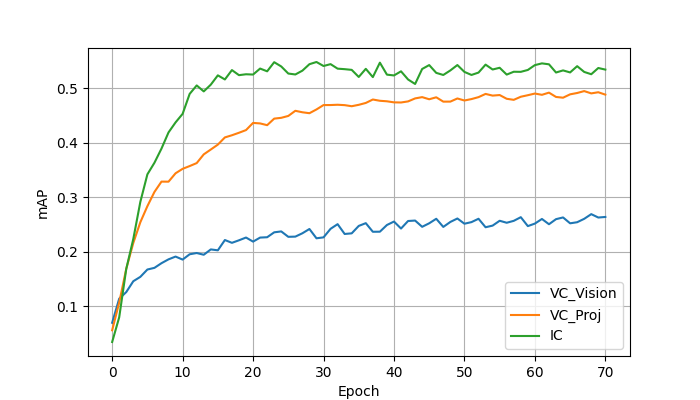
\includegraphics[width=1.0\textwidth]{assets/imgs/5_1_BackboneSelection.pgf}
    \resizebox{1.0\textwidth}{!}{%% Creator: Matplotlib, PGF backend
%%
%% To include the figure in your LaTeX document, write
%%   \input{<filename>.pgf}
%%
%% Make sure the required packages are loaded in your preamble
%%   \usepackage{pgf}
%%
%% and, on pdftex
%%   \usepackage[utf8]{inputenc}\DeclareUnicodeCharacter{2212}{-}
%%
%% or, on luatex and xetex
%%   \usepackage{unicode-math}
%%
%% Figures using additional raster images can only be included by \input if
%% they are in the same directory as the main LaTeX file. For loading figures
%% from other directories you can use the `import` package
%%   \usepackage{import}
%%
%% and then include the figures with
%%   \import{<path to file>}{<filename>.pgf}
%%
%% Matplotlib used the following preamble
%%
\begingroup%
\makeatletter%
\begin{pgfpicture}%
\pgfpathrectangle{\pgfpointorigin}{\pgfqpoint{7.000000in}{4.000000in}}%
\pgfusepath{use as bounding box, clip}%
\begin{pgfscope}%
\pgfsetbuttcap%
\pgfsetmiterjoin%
\definecolor{currentfill}{rgb}{1.000000,1.000000,1.000000}%
\pgfsetfillcolor{currentfill}%
\pgfsetlinewidth{0.000000pt}%
\definecolor{currentstroke}{rgb}{1.000000,1.000000,1.000000}%
\pgfsetstrokecolor{currentstroke}%
\pgfsetdash{}{0pt}%
\pgfpathmoveto{\pgfqpoint{0.000000in}{0.000000in}}%
\pgfpathlineto{\pgfqpoint{7.000000in}{0.000000in}}%
\pgfpathlineto{\pgfqpoint{7.000000in}{4.000000in}}%
\pgfpathlineto{\pgfqpoint{0.000000in}{4.000000in}}%
\pgfpathclose%
\pgfusepath{fill}%
\end{pgfscope}%
\begin{pgfscope}%
\pgfsetbuttcap%
\pgfsetmiterjoin%
\definecolor{currentfill}{rgb}{1.000000,1.000000,1.000000}%
\pgfsetfillcolor{currentfill}%
\pgfsetlinewidth{0.000000pt}%
\definecolor{currentstroke}{rgb}{0.000000,0.000000,0.000000}%
\pgfsetstrokecolor{currentstroke}%
\pgfsetstrokeopacity{0.000000}%
\pgfsetdash{}{0pt}%
\pgfpathmoveto{\pgfqpoint{0.875000in}{0.440000in}}%
\pgfpathlineto{\pgfqpoint{6.300000in}{0.440000in}}%
\pgfpathlineto{\pgfqpoint{6.300000in}{3.520000in}}%
\pgfpathlineto{\pgfqpoint{0.875000in}{3.520000in}}%
\pgfpathclose%
\pgfusepath{fill}%
\end{pgfscope}%
\begin{pgfscope}%
\pgfpathrectangle{\pgfqpoint{0.875000in}{0.440000in}}{\pgfqpoint{5.425000in}{3.080000in}}%
\pgfusepath{clip}%
\pgfsetrectcap%
\pgfsetroundjoin%
\pgfsetlinewidth{0.803000pt}%
\definecolor{currentstroke}{rgb}{0.690196,0.690196,0.690196}%
\pgfsetstrokecolor{currentstroke}%
\pgfsetdash{}{0pt}%
\pgfpathmoveto{\pgfqpoint{1.121591in}{0.440000in}}%
\pgfpathlineto{\pgfqpoint{1.121591in}{3.520000in}}%
\pgfusepath{stroke}%
\end{pgfscope}%
\begin{pgfscope}%
\pgfsetbuttcap%
\pgfsetroundjoin%
\definecolor{currentfill}{rgb}{0.000000,0.000000,0.000000}%
\pgfsetfillcolor{currentfill}%
\pgfsetlinewidth{0.803000pt}%
\definecolor{currentstroke}{rgb}{0.000000,0.000000,0.000000}%
\pgfsetstrokecolor{currentstroke}%
\pgfsetdash{}{0pt}%
\pgfsys@defobject{currentmarker}{\pgfqpoint{0.000000in}{-0.048611in}}{\pgfqpoint{0.000000in}{0.000000in}}{%
\pgfpathmoveto{\pgfqpoint{0.000000in}{0.000000in}}%
\pgfpathlineto{\pgfqpoint{0.000000in}{-0.048611in}}%
\pgfusepath{stroke,fill}%
}%
\begin{pgfscope}%
\pgfsys@transformshift{1.121591in}{0.440000in}%
\pgfsys@useobject{currentmarker}{}%
\end{pgfscope}%
\end{pgfscope}%
\begin{pgfscope}%
\definecolor{textcolor}{rgb}{0.000000,0.000000,0.000000}%
\pgfsetstrokecolor{textcolor}%
\pgfsetfillcolor{textcolor}%
\pgftext[x=1.121591in,y=0.342778in,,top]{\color{textcolor}\rmfamily\fontsize{10.000000}{12.000000}\selectfont \(\displaystyle {0}\)}%
\end{pgfscope}%
\begin{pgfscope}%
\pgfpathrectangle{\pgfqpoint{0.875000in}{0.440000in}}{\pgfqpoint{5.425000in}{3.080000in}}%
\pgfusepath{clip}%
\pgfsetrectcap%
\pgfsetroundjoin%
\pgfsetlinewidth{0.803000pt}%
\definecolor{currentstroke}{rgb}{0.690196,0.690196,0.690196}%
\pgfsetstrokecolor{currentstroke}%
\pgfsetdash{}{0pt}%
\pgfpathmoveto{\pgfqpoint{1.738068in}{0.440000in}}%
\pgfpathlineto{\pgfqpoint{1.738068in}{3.520000in}}%
\pgfusepath{stroke}%
\end{pgfscope}%
\begin{pgfscope}%
\pgfsetbuttcap%
\pgfsetroundjoin%
\definecolor{currentfill}{rgb}{0.000000,0.000000,0.000000}%
\pgfsetfillcolor{currentfill}%
\pgfsetlinewidth{0.803000pt}%
\definecolor{currentstroke}{rgb}{0.000000,0.000000,0.000000}%
\pgfsetstrokecolor{currentstroke}%
\pgfsetdash{}{0pt}%
\pgfsys@defobject{currentmarker}{\pgfqpoint{0.000000in}{-0.048611in}}{\pgfqpoint{0.000000in}{0.000000in}}{%
\pgfpathmoveto{\pgfqpoint{0.000000in}{0.000000in}}%
\pgfpathlineto{\pgfqpoint{0.000000in}{-0.048611in}}%
\pgfusepath{stroke,fill}%
}%
\begin{pgfscope}%
\pgfsys@transformshift{1.738068in}{0.440000in}%
\pgfsys@useobject{currentmarker}{}%
\end{pgfscope}%
\end{pgfscope}%
\begin{pgfscope}%
\definecolor{textcolor}{rgb}{0.000000,0.000000,0.000000}%
\pgfsetstrokecolor{textcolor}%
\pgfsetfillcolor{textcolor}%
\pgftext[x=1.738068in,y=0.342778in,,top]{\color{textcolor}\rmfamily\fontsize{10.000000}{12.000000}\selectfont \(\displaystyle {10}\)}%
\end{pgfscope}%
\begin{pgfscope}%
\pgfpathrectangle{\pgfqpoint{0.875000in}{0.440000in}}{\pgfqpoint{5.425000in}{3.080000in}}%
\pgfusepath{clip}%
\pgfsetrectcap%
\pgfsetroundjoin%
\pgfsetlinewidth{0.803000pt}%
\definecolor{currentstroke}{rgb}{0.690196,0.690196,0.690196}%
\pgfsetstrokecolor{currentstroke}%
\pgfsetdash{}{0pt}%
\pgfpathmoveto{\pgfqpoint{2.354545in}{0.440000in}}%
\pgfpathlineto{\pgfqpoint{2.354545in}{3.520000in}}%
\pgfusepath{stroke}%
\end{pgfscope}%
\begin{pgfscope}%
\pgfsetbuttcap%
\pgfsetroundjoin%
\definecolor{currentfill}{rgb}{0.000000,0.000000,0.000000}%
\pgfsetfillcolor{currentfill}%
\pgfsetlinewidth{0.803000pt}%
\definecolor{currentstroke}{rgb}{0.000000,0.000000,0.000000}%
\pgfsetstrokecolor{currentstroke}%
\pgfsetdash{}{0pt}%
\pgfsys@defobject{currentmarker}{\pgfqpoint{0.000000in}{-0.048611in}}{\pgfqpoint{0.000000in}{0.000000in}}{%
\pgfpathmoveto{\pgfqpoint{0.000000in}{0.000000in}}%
\pgfpathlineto{\pgfqpoint{0.000000in}{-0.048611in}}%
\pgfusepath{stroke,fill}%
}%
\begin{pgfscope}%
\pgfsys@transformshift{2.354545in}{0.440000in}%
\pgfsys@useobject{currentmarker}{}%
\end{pgfscope}%
\end{pgfscope}%
\begin{pgfscope}%
\definecolor{textcolor}{rgb}{0.000000,0.000000,0.000000}%
\pgfsetstrokecolor{textcolor}%
\pgfsetfillcolor{textcolor}%
\pgftext[x=2.354545in,y=0.342778in,,top]{\color{textcolor}\rmfamily\fontsize{10.000000}{12.000000}\selectfont \(\displaystyle {20}\)}%
\end{pgfscope}%
\begin{pgfscope}%
\pgfpathrectangle{\pgfqpoint{0.875000in}{0.440000in}}{\pgfqpoint{5.425000in}{3.080000in}}%
\pgfusepath{clip}%
\pgfsetrectcap%
\pgfsetroundjoin%
\pgfsetlinewidth{0.803000pt}%
\definecolor{currentstroke}{rgb}{0.690196,0.690196,0.690196}%
\pgfsetstrokecolor{currentstroke}%
\pgfsetdash{}{0pt}%
\pgfpathmoveto{\pgfqpoint{2.971023in}{0.440000in}}%
\pgfpathlineto{\pgfqpoint{2.971023in}{3.520000in}}%
\pgfusepath{stroke}%
\end{pgfscope}%
\begin{pgfscope}%
\pgfsetbuttcap%
\pgfsetroundjoin%
\definecolor{currentfill}{rgb}{0.000000,0.000000,0.000000}%
\pgfsetfillcolor{currentfill}%
\pgfsetlinewidth{0.803000pt}%
\definecolor{currentstroke}{rgb}{0.000000,0.000000,0.000000}%
\pgfsetstrokecolor{currentstroke}%
\pgfsetdash{}{0pt}%
\pgfsys@defobject{currentmarker}{\pgfqpoint{0.000000in}{-0.048611in}}{\pgfqpoint{0.000000in}{0.000000in}}{%
\pgfpathmoveto{\pgfqpoint{0.000000in}{0.000000in}}%
\pgfpathlineto{\pgfqpoint{0.000000in}{-0.048611in}}%
\pgfusepath{stroke,fill}%
}%
\begin{pgfscope}%
\pgfsys@transformshift{2.971023in}{0.440000in}%
\pgfsys@useobject{currentmarker}{}%
\end{pgfscope}%
\end{pgfscope}%
\begin{pgfscope}%
\definecolor{textcolor}{rgb}{0.000000,0.000000,0.000000}%
\pgfsetstrokecolor{textcolor}%
\pgfsetfillcolor{textcolor}%
\pgftext[x=2.971023in,y=0.342778in,,top]{\color{textcolor}\rmfamily\fontsize{10.000000}{12.000000}\selectfont \(\displaystyle {30}\)}%
\end{pgfscope}%
\begin{pgfscope}%
\pgfpathrectangle{\pgfqpoint{0.875000in}{0.440000in}}{\pgfqpoint{5.425000in}{3.080000in}}%
\pgfusepath{clip}%
\pgfsetrectcap%
\pgfsetroundjoin%
\pgfsetlinewidth{0.803000pt}%
\definecolor{currentstroke}{rgb}{0.690196,0.690196,0.690196}%
\pgfsetstrokecolor{currentstroke}%
\pgfsetdash{}{0pt}%
\pgfpathmoveto{\pgfqpoint{3.587500in}{0.440000in}}%
\pgfpathlineto{\pgfqpoint{3.587500in}{3.520000in}}%
\pgfusepath{stroke}%
\end{pgfscope}%
\begin{pgfscope}%
\pgfsetbuttcap%
\pgfsetroundjoin%
\definecolor{currentfill}{rgb}{0.000000,0.000000,0.000000}%
\pgfsetfillcolor{currentfill}%
\pgfsetlinewidth{0.803000pt}%
\definecolor{currentstroke}{rgb}{0.000000,0.000000,0.000000}%
\pgfsetstrokecolor{currentstroke}%
\pgfsetdash{}{0pt}%
\pgfsys@defobject{currentmarker}{\pgfqpoint{0.000000in}{-0.048611in}}{\pgfqpoint{0.000000in}{0.000000in}}{%
\pgfpathmoveto{\pgfqpoint{0.000000in}{0.000000in}}%
\pgfpathlineto{\pgfqpoint{0.000000in}{-0.048611in}}%
\pgfusepath{stroke,fill}%
}%
\begin{pgfscope}%
\pgfsys@transformshift{3.587500in}{0.440000in}%
\pgfsys@useobject{currentmarker}{}%
\end{pgfscope}%
\end{pgfscope}%
\begin{pgfscope}%
\definecolor{textcolor}{rgb}{0.000000,0.000000,0.000000}%
\pgfsetstrokecolor{textcolor}%
\pgfsetfillcolor{textcolor}%
\pgftext[x=3.587500in,y=0.342778in,,top]{\color{textcolor}\rmfamily\fontsize{10.000000}{12.000000}\selectfont \(\displaystyle {40}\)}%
\end{pgfscope}%
\begin{pgfscope}%
\pgfpathrectangle{\pgfqpoint{0.875000in}{0.440000in}}{\pgfqpoint{5.425000in}{3.080000in}}%
\pgfusepath{clip}%
\pgfsetrectcap%
\pgfsetroundjoin%
\pgfsetlinewidth{0.803000pt}%
\definecolor{currentstroke}{rgb}{0.690196,0.690196,0.690196}%
\pgfsetstrokecolor{currentstroke}%
\pgfsetdash{}{0pt}%
\pgfpathmoveto{\pgfqpoint{4.203977in}{0.440000in}}%
\pgfpathlineto{\pgfqpoint{4.203977in}{3.520000in}}%
\pgfusepath{stroke}%
\end{pgfscope}%
\begin{pgfscope}%
\pgfsetbuttcap%
\pgfsetroundjoin%
\definecolor{currentfill}{rgb}{0.000000,0.000000,0.000000}%
\pgfsetfillcolor{currentfill}%
\pgfsetlinewidth{0.803000pt}%
\definecolor{currentstroke}{rgb}{0.000000,0.000000,0.000000}%
\pgfsetstrokecolor{currentstroke}%
\pgfsetdash{}{0pt}%
\pgfsys@defobject{currentmarker}{\pgfqpoint{0.000000in}{-0.048611in}}{\pgfqpoint{0.000000in}{0.000000in}}{%
\pgfpathmoveto{\pgfqpoint{0.000000in}{0.000000in}}%
\pgfpathlineto{\pgfqpoint{0.000000in}{-0.048611in}}%
\pgfusepath{stroke,fill}%
}%
\begin{pgfscope}%
\pgfsys@transformshift{4.203977in}{0.440000in}%
\pgfsys@useobject{currentmarker}{}%
\end{pgfscope}%
\end{pgfscope}%
\begin{pgfscope}%
\definecolor{textcolor}{rgb}{0.000000,0.000000,0.000000}%
\pgfsetstrokecolor{textcolor}%
\pgfsetfillcolor{textcolor}%
\pgftext[x=4.203977in,y=0.342778in,,top]{\color{textcolor}\rmfamily\fontsize{10.000000}{12.000000}\selectfont \(\displaystyle {50}\)}%
\end{pgfscope}%
\begin{pgfscope}%
\pgfpathrectangle{\pgfqpoint{0.875000in}{0.440000in}}{\pgfqpoint{5.425000in}{3.080000in}}%
\pgfusepath{clip}%
\pgfsetrectcap%
\pgfsetroundjoin%
\pgfsetlinewidth{0.803000pt}%
\definecolor{currentstroke}{rgb}{0.690196,0.690196,0.690196}%
\pgfsetstrokecolor{currentstroke}%
\pgfsetdash{}{0pt}%
\pgfpathmoveto{\pgfqpoint{4.820455in}{0.440000in}}%
\pgfpathlineto{\pgfqpoint{4.820455in}{3.520000in}}%
\pgfusepath{stroke}%
\end{pgfscope}%
\begin{pgfscope}%
\pgfsetbuttcap%
\pgfsetroundjoin%
\definecolor{currentfill}{rgb}{0.000000,0.000000,0.000000}%
\pgfsetfillcolor{currentfill}%
\pgfsetlinewidth{0.803000pt}%
\definecolor{currentstroke}{rgb}{0.000000,0.000000,0.000000}%
\pgfsetstrokecolor{currentstroke}%
\pgfsetdash{}{0pt}%
\pgfsys@defobject{currentmarker}{\pgfqpoint{0.000000in}{-0.048611in}}{\pgfqpoint{0.000000in}{0.000000in}}{%
\pgfpathmoveto{\pgfqpoint{0.000000in}{0.000000in}}%
\pgfpathlineto{\pgfqpoint{0.000000in}{-0.048611in}}%
\pgfusepath{stroke,fill}%
}%
\begin{pgfscope}%
\pgfsys@transformshift{4.820455in}{0.440000in}%
\pgfsys@useobject{currentmarker}{}%
\end{pgfscope}%
\end{pgfscope}%
\begin{pgfscope}%
\definecolor{textcolor}{rgb}{0.000000,0.000000,0.000000}%
\pgfsetstrokecolor{textcolor}%
\pgfsetfillcolor{textcolor}%
\pgftext[x=4.820455in,y=0.342778in,,top]{\color{textcolor}\rmfamily\fontsize{10.000000}{12.000000}\selectfont \(\displaystyle {60}\)}%
\end{pgfscope}%
\begin{pgfscope}%
\pgfpathrectangle{\pgfqpoint{0.875000in}{0.440000in}}{\pgfqpoint{5.425000in}{3.080000in}}%
\pgfusepath{clip}%
\pgfsetrectcap%
\pgfsetroundjoin%
\pgfsetlinewidth{0.803000pt}%
\definecolor{currentstroke}{rgb}{0.690196,0.690196,0.690196}%
\pgfsetstrokecolor{currentstroke}%
\pgfsetdash{}{0pt}%
\pgfpathmoveto{\pgfqpoint{5.436932in}{0.440000in}}%
\pgfpathlineto{\pgfqpoint{5.436932in}{3.520000in}}%
\pgfusepath{stroke}%
\end{pgfscope}%
\begin{pgfscope}%
\pgfsetbuttcap%
\pgfsetroundjoin%
\definecolor{currentfill}{rgb}{0.000000,0.000000,0.000000}%
\pgfsetfillcolor{currentfill}%
\pgfsetlinewidth{0.803000pt}%
\definecolor{currentstroke}{rgb}{0.000000,0.000000,0.000000}%
\pgfsetstrokecolor{currentstroke}%
\pgfsetdash{}{0pt}%
\pgfsys@defobject{currentmarker}{\pgfqpoint{0.000000in}{-0.048611in}}{\pgfqpoint{0.000000in}{0.000000in}}{%
\pgfpathmoveto{\pgfqpoint{0.000000in}{0.000000in}}%
\pgfpathlineto{\pgfqpoint{0.000000in}{-0.048611in}}%
\pgfusepath{stroke,fill}%
}%
\begin{pgfscope}%
\pgfsys@transformshift{5.436932in}{0.440000in}%
\pgfsys@useobject{currentmarker}{}%
\end{pgfscope}%
\end{pgfscope}%
\begin{pgfscope}%
\definecolor{textcolor}{rgb}{0.000000,0.000000,0.000000}%
\pgfsetstrokecolor{textcolor}%
\pgfsetfillcolor{textcolor}%
\pgftext[x=5.436932in,y=0.342778in,,top]{\color{textcolor}\rmfamily\fontsize{10.000000}{12.000000}\selectfont \(\displaystyle {70}\)}%
\end{pgfscope}%
\begin{pgfscope}%
\pgfpathrectangle{\pgfqpoint{0.875000in}{0.440000in}}{\pgfqpoint{5.425000in}{3.080000in}}%
\pgfusepath{clip}%
\pgfsetrectcap%
\pgfsetroundjoin%
\pgfsetlinewidth{0.803000pt}%
\definecolor{currentstroke}{rgb}{0.690196,0.690196,0.690196}%
\pgfsetstrokecolor{currentstroke}%
\pgfsetdash{}{0pt}%
\pgfpathmoveto{\pgfqpoint{6.053409in}{0.440000in}}%
\pgfpathlineto{\pgfqpoint{6.053409in}{3.520000in}}%
\pgfusepath{stroke}%
\end{pgfscope}%
\begin{pgfscope}%
\pgfsetbuttcap%
\pgfsetroundjoin%
\definecolor{currentfill}{rgb}{0.000000,0.000000,0.000000}%
\pgfsetfillcolor{currentfill}%
\pgfsetlinewidth{0.803000pt}%
\definecolor{currentstroke}{rgb}{0.000000,0.000000,0.000000}%
\pgfsetstrokecolor{currentstroke}%
\pgfsetdash{}{0pt}%
\pgfsys@defobject{currentmarker}{\pgfqpoint{0.000000in}{-0.048611in}}{\pgfqpoint{0.000000in}{0.000000in}}{%
\pgfpathmoveto{\pgfqpoint{0.000000in}{0.000000in}}%
\pgfpathlineto{\pgfqpoint{0.000000in}{-0.048611in}}%
\pgfusepath{stroke,fill}%
}%
\begin{pgfscope}%
\pgfsys@transformshift{6.053409in}{0.440000in}%
\pgfsys@useobject{currentmarker}{}%
\end{pgfscope}%
\end{pgfscope}%
\begin{pgfscope}%
\definecolor{textcolor}{rgb}{0.000000,0.000000,0.000000}%
\pgfsetstrokecolor{textcolor}%
\pgfsetfillcolor{textcolor}%
\pgftext[x=6.053409in,y=0.342778in,,top]{\color{textcolor}\rmfamily\fontsize{10.000000}{12.000000}\selectfont \(\displaystyle {80}\)}%
\end{pgfscope}%
\begin{pgfscope}%
\definecolor{textcolor}{rgb}{0.000000,0.000000,0.000000}%
\pgfsetstrokecolor{textcolor}%
\pgfsetfillcolor{textcolor}%
\pgftext[x=3.587500in,y=0.163766in,,top]{\color{textcolor}\rmfamily\fontsize{10.000000}{12.000000}\selectfont Epoch}%
\end{pgfscope}%
\begin{pgfscope}%
\pgfpathrectangle{\pgfqpoint{0.875000in}{0.440000in}}{\pgfqpoint{5.425000in}{3.080000in}}%
\pgfusepath{clip}%
\pgfsetrectcap%
\pgfsetroundjoin%
\pgfsetlinewidth{0.803000pt}%
\definecolor{currentstroke}{rgb}{0.690196,0.690196,0.690196}%
\pgfsetstrokecolor{currentstroke}%
\pgfsetdash{}{0pt}%
\pgfpathmoveto{\pgfqpoint{0.875000in}{0.953310in}}%
\pgfpathlineto{\pgfqpoint{6.300000in}{0.953310in}}%
\pgfusepath{stroke}%
\end{pgfscope}%
\begin{pgfscope}%
\pgfsetbuttcap%
\pgfsetroundjoin%
\definecolor{currentfill}{rgb}{0.000000,0.000000,0.000000}%
\pgfsetfillcolor{currentfill}%
\pgfsetlinewidth{0.803000pt}%
\definecolor{currentstroke}{rgb}{0.000000,0.000000,0.000000}%
\pgfsetstrokecolor{currentstroke}%
\pgfsetdash{}{0pt}%
\pgfsys@defobject{currentmarker}{\pgfqpoint{-0.048611in}{0.000000in}}{\pgfqpoint{0.000000in}{0.000000in}}{%
\pgfpathmoveto{\pgfqpoint{0.000000in}{0.000000in}}%
\pgfpathlineto{\pgfqpoint{-0.048611in}{0.000000in}}%
\pgfusepath{stroke,fill}%
}%
\begin{pgfscope}%
\pgfsys@transformshift{0.875000in}{0.953310in}%
\pgfsys@useobject{currentmarker}{}%
\end{pgfscope}%
\end{pgfscope}%
\begin{pgfscope}%
\definecolor{textcolor}{rgb}{0.000000,0.000000,0.000000}%
\pgfsetstrokecolor{textcolor}%
\pgfsetfillcolor{textcolor}%
\pgftext[x=0.600308in, y=0.905085in, left, base]{\color{textcolor}\rmfamily\fontsize{10.000000}{12.000000}\selectfont \(\displaystyle {0.1}\)}%
\end{pgfscope}%
\begin{pgfscope}%
\pgfpathrectangle{\pgfqpoint{0.875000in}{0.440000in}}{\pgfqpoint{5.425000in}{3.080000in}}%
\pgfusepath{clip}%
\pgfsetrectcap%
\pgfsetroundjoin%
\pgfsetlinewidth{0.803000pt}%
\definecolor{currentstroke}{rgb}{0.690196,0.690196,0.690196}%
\pgfsetstrokecolor{currentstroke}%
\pgfsetdash{}{0pt}%
\pgfpathmoveto{\pgfqpoint{0.875000in}{1.500339in}}%
\pgfpathlineto{\pgfqpoint{6.300000in}{1.500339in}}%
\pgfusepath{stroke}%
\end{pgfscope}%
\begin{pgfscope}%
\pgfsetbuttcap%
\pgfsetroundjoin%
\definecolor{currentfill}{rgb}{0.000000,0.000000,0.000000}%
\pgfsetfillcolor{currentfill}%
\pgfsetlinewidth{0.803000pt}%
\definecolor{currentstroke}{rgb}{0.000000,0.000000,0.000000}%
\pgfsetstrokecolor{currentstroke}%
\pgfsetdash{}{0pt}%
\pgfsys@defobject{currentmarker}{\pgfqpoint{-0.048611in}{0.000000in}}{\pgfqpoint{0.000000in}{0.000000in}}{%
\pgfpathmoveto{\pgfqpoint{0.000000in}{0.000000in}}%
\pgfpathlineto{\pgfqpoint{-0.048611in}{0.000000in}}%
\pgfusepath{stroke,fill}%
}%
\begin{pgfscope}%
\pgfsys@transformshift{0.875000in}{1.500339in}%
\pgfsys@useobject{currentmarker}{}%
\end{pgfscope}%
\end{pgfscope}%
\begin{pgfscope}%
\definecolor{textcolor}{rgb}{0.000000,0.000000,0.000000}%
\pgfsetstrokecolor{textcolor}%
\pgfsetfillcolor{textcolor}%
\pgftext[x=0.600308in, y=1.452113in, left, base]{\color{textcolor}\rmfamily\fontsize{10.000000}{12.000000}\selectfont \(\displaystyle {0.2}\)}%
\end{pgfscope}%
\begin{pgfscope}%
\pgfpathrectangle{\pgfqpoint{0.875000in}{0.440000in}}{\pgfqpoint{5.425000in}{3.080000in}}%
\pgfusepath{clip}%
\pgfsetrectcap%
\pgfsetroundjoin%
\pgfsetlinewidth{0.803000pt}%
\definecolor{currentstroke}{rgb}{0.690196,0.690196,0.690196}%
\pgfsetstrokecolor{currentstroke}%
\pgfsetdash{}{0pt}%
\pgfpathmoveto{\pgfqpoint{0.875000in}{2.047367in}}%
\pgfpathlineto{\pgfqpoint{6.300000in}{2.047367in}}%
\pgfusepath{stroke}%
\end{pgfscope}%
\begin{pgfscope}%
\pgfsetbuttcap%
\pgfsetroundjoin%
\definecolor{currentfill}{rgb}{0.000000,0.000000,0.000000}%
\pgfsetfillcolor{currentfill}%
\pgfsetlinewidth{0.803000pt}%
\definecolor{currentstroke}{rgb}{0.000000,0.000000,0.000000}%
\pgfsetstrokecolor{currentstroke}%
\pgfsetdash{}{0pt}%
\pgfsys@defobject{currentmarker}{\pgfqpoint{-0.048611in}{0.000000in}}{\pgfqpoint{0.000000in}{0.000000in}}{%
\pgfpathmoveto{\pgfqpoint{0.000000in}{0.000000in}}%
\pgfpathlineto{\pgfqpoint{-0.048611in}{0.000000in}}%
\pgfusepath{stroke,fill}%
}%
\begin{pgfscope}%
\pgfsys@transformshift{0.875000in}{2.047367in}%
\pgfsys@useobject{currentmarker}{}%
\end{pgfscope}%
\end{pgfscope}%
\begin{pgfscope}%
\definecolor{textcolor}{rgb}{0.000000,0.000000,0.000000}%
\pgfsetstrokecolor{textcolor}%
\pgfsetfillcolor{textcolor}%
\pgftext[x=0.600308in, y=1.999141in, left, base]{\color{textcolor}\rmfamily\fontsize{10.000000}{12.000000}\selectfont \(\displaystyle {0.3}\)}%
\end{pgfscope}%
\begin{pgfscope}%
\pgfpathrectangle{\pgfqpoint{0.875000in}{0.440000in}}{\pgfqpoint{5.425000in}{3.080000in}}%
\pgfusepath{clip}%
\pgfsetrectcap%
\pgfsetroundjoin%
\pgfsetlinewidth{0.803000pt}%
\definecolor{currentstroke}{rgb}{0.690196,0.690196,0.690196}%
\pgfsetstrokecolor{currentstroke}%
\pgfsetdash{}{0pt}%
\pgfpathmoveto{\pgfqpoint{0.875000in}{2.594395in}}%
\pgfpathlineto{\pgfqpoint{6.300000in}{2.594395in}}%
\pgfusepath{stroke}%
\end{pgfscope}%
\begin{pgfscope}%
\pgfsetbuttcap%
\pgfsetroundjoin%
\definecolor{currentfill}{rgb}{0.000000,0.000000,0.000000}%
\pgfsetfillcolor{currentfill}%
\pgfsetlinewidth{0.803000pt}%
\definecolor{currentstroke}{rgb}{0.000000,0.000000,0.000000}%
\pgfsetstrokecolor{currentstroke}%
\pgfsetdash{}{0pt}%
\pgfsys@defobject{currentmarker}{\pgfqpoint{-0.048611in}{0.000000in}}{\pgfqpoint{0.000000in}{0.000000in}}{%
\pgfpathmoveto{\pgfqpoint{0.000000in}{0.000000in}}%
\pgfpathlineto{\pgfqpoint{-0.048611in}{0.000000in}}%
\pgfusepath{stroke,fill}%
}%
\begin{pgfscope}%
\pgfsys@transformshift{0.875000in}{2.594395in}%
\pgfsys@useobject{currentmarker}{}%
\end{pgfscope}%
\end{pgfscope}%
\begin{pgfscope}%
\definecolor{textcolor}{rgb}{0.000000,0.000000,0.000000}%
\pgfsetstrokecolor{textcolor}%
\pgfsetfillcolor{textcolor}%
\pgftext[x=0.600308in, y=2.546170in, left, base]{\color{textcolor}\rmfamily\fontsize{10.000000}{12.000000}\selectfont \(\displaystyle {0.4}\)}%
\end{pgfscope}%
\begin{pgfscope}%
\pgfpathrectangle{\pgfqpoint{0.875000in}{0.440000in}}{\pgfqpoint{5.425000in}{3.080000in}}%
\pgfusepath{clip}%
\pgfsetrectcap%
\pgfsetroundjoin%
\pgfsetlinewidth{0.803000pt}%
\definecolor{currentstroke}{rgb}{0.690196,0.690196,0.690196}%
\pgfsetstrokecolor{currentstroke}%
\pgfsetdash{}{0pt}%
\pgfpathmoveto{\pgfqpoint{0.875000in}{3.141423in}}%
\pgfpathlineto{\pgfqpoint{6.300000in}{3.141423in}}%
\pgfusepath{stroke}%
\end{pgfscope}%
\begin{pgfscope}%
\pgfsetbuttcap%
\pgfsetroundjoin%
\definecolor{currentfill}{rgb}{0.000000,0.000000,0.000000}%
\pgfsetfillcolor{currentfill}%
\pgfsetlinewidth{0.803000pt}%
\definecolor{currentstroke}{rgb}{0.000000,0.000000,0.000000}%
\pgfsetstrokecolor{currentstroke}%
\pgfsetdash{}{0pt}%
\pgfsys@defobject{currentmarker}{\pgfqpoint{-0.048611in}{0.000000in}}{\pgfqpoint{0.000000in}{0.000000in}}{%
\pgfpathmoveto{\pgfqpoint{0.000000in}{0.000000in}}%
\pgfpathlineto{\pgfqpoint{-0.048611in}{0.000000in}}%
\pgfusepath{stroke,fill}%
}%
\begin{pgfscope}%
\pgfsys@transformshift{0.875000in}{3.141423in}%
\pgfsys@useobject{currentmarker}{}%
\end{pgfscope}%
\end{pgfscope}%
\begin{pgfscope}%
\definecolor{textcolor}{rgb}{0.000000,0.000000,0.000000}%
\pgfsetstrokecolor{textcolor}%
\pgfsetfillcolor{textcolor}%
\pgftext[x=0.600308in, y=3.093198in, left, base]{\color{textcolor}\rmfamily\fontsize{10.000000}{12.000000}\selectfont \(\displaystyle {0.5}\)}%
\end{pgfscope}%
\begin{pgfscope}%
\definecolor{textcolor}{rgb}{0.000000,0.000000,0.000000}%
\pgfsetstrokecolor{textcolor}%
\pgfsetfillcolor{textcolor}%
\pgftext[x=0.544752in,y=1.980000in,,bottom,rotate=90.000000]{\color{textcolor}\rmfamily\fontsize{10.000000}{12.000000}\selectfont mAP}%
\end{pgfscope}%
\begin{pgfscope}%
\pgfpathrectangle{\pgfqpoint{0.875000in}{0.440000in}}{\pgfqpoint{5.425000in}{3.080000in}}%
\pgfusepath{clip}%
\pgfsetrectcap%
\pgfsetroundjoin%
\pgfsetlinewidth{1.505625pt}%
\definecolor{currentstroke}{rgb}{0.121569,0.466667,0.705882}%
\pgfsetstrokecolor{currentstroke}%
\pgfsetdash{}{0pt}%
\pgfpathmoveto{\pgfqpoint{1.121591in}{0.790032in}}%
\pgfpathlineto{\pgfqpoint{1.183239in}{1.031670in}}%
\pgfpathlineto{\pgfqpoint{1.244886in}{1.097626in}}%
\pgfpathlineto{\pgfqpoint{1.306534in}{1.206504in}}%
\pgfpathlineto{\pgfqpoint{1.368182in}{1.250288in}}%
\pgfpathlineto{\pgfqpoint{1.429830in}{1.323820in}}%
\pgfpathlineto{\pgfqpoint{1.491477in}{1.340464in}}%
\pgfpathlineto{\pgfqpoint{1.553125in}{1.387178in}}%
\pgfpathlineto{\pgfqpoint{1.614773in}{1.425803in}}%
\pgfpathlineto{\pgfqpoint{1.676420in}{1.453569in}}%
\pgfpathlineto{\pgfqpoint{1.738068in}{1.423318in}}%
\pgfpathlineto{\pgfqpoint{1.799716in}{1.476685in}}%
\pgfpathlineto{\pgfqpoint{1.861364in}{1.489150in}}%
\pgfpathlineto{\pgfqpoint{1.923011in}{1.471761in}}%
\pgfpathlineto{\pgfqpoint{1.984659in}{1.525217in}}%
\pgfpathlineto{\pgfqpoint{2.046307in}{1.516235in}}%
\pgfpathlineto{\pgfqpoint{2.107955in}{1.619298in}}%
\pgfpathlineto{\pgfqpoint{2.169602in}{1.591322in}}%
\pgfpathlineto{\pgfqpoint{2.231250in}{1.616672in}}%
\pgfpathlineto{\pgfqpoint{2.292898in}{1.644373in}}%
\pgfpathlineto{\pgfqpoint{2.354545in}{1.603481in}}%
\pgfpathlineto{\pgfqpoint{2.416193in}{1.643884in}}%
\pgfpathlineto{\pgfqpoint{2.477841in}{1.647356in}}%
\pgfpathlineto{\pgfqpoint{2.539489in}{1.696610in}}%
\pgfpathlineto{\pgfqpoint{2.601136in}{1.705648in}}%
\pgfpathlineto{\pgfqpoint{2.662784in}{1.651535in}}%
\pgfpathlineto{\pgfqpoint{2.724432in}{1.653559in}}%
\pgfpathlineto{\pgfqpoint{2.786080in}{1.687076in}}%
\pgfpathlineto{\pgfqpoint{2.847727in}{1.729877in}}%
\pgfpathlineto{\pgfqpoint{2.909375in}{1.636803in}}%
\pgfpathlineto{\pgfqpoint{2.971023in}{1.646038in}}%
\pgfpathlineto{\pgfqpoint{3.032670in}{1.731818in}}%
\pgfpathlineto{\pgfqpoint{3.094318in}{1.778419in}}%
\pgfpathlineto{\pgfqpoint{3.155966in}{1.680050in}}%
\pgfpathlineto{\pgfqpoint{3.217614in}{1.686401in}}%
\pgfpathlineto{\pgfqpoint{3.279261in}{1.760793in}}%
\pgfpathlineto{\pgfqpoint{3.340909in}{1.788454in}}%
\pgfpathlineto{\pgfqpoint{3.402557in}{1.702096in}}%
\pgfpathlineto{\pgfqpoint{3.464205in}{1.702846in}}%
\pgfpathlineto{\pgfqpoint{3.525852in}{1.770005in}}%
\pgfpathlineto{\pgfqpoint{3.587500in}{1.804481in}}%
\pgfpathlineto{\pgfqpoint{3.649148in}{1.734448in}}%
\pgfpathlineto{\pgfqpoint{3.710795in}{1.810009in}}%
\pgfpathlineto{\pgfqpoint{3.772443in}{1.814459in}}%
\pgfpathlineto{\pgfqpoint{3.834091in}{1.751825in}}%
\pgfpathlineto{\pgfqpoint{3.895739in}{1.787175in}}%
\pgfpathlineto{\pgfqpoint{3.957386in}{1.832313in}}%
\pgfpathlineto{\pgfqpoint{4.019034in}{1.750698in}}%
\pgfpathlineto{\pgfqpoint{4.080682in}{1.800504in}}%
\pgfpathlineto{\pgfqpoint{4.142330in}{1.835156in}}%
\pgfpathlineto{\pgfqpoint{4.203977in}{1.782828in}}%
\pgfpathlineto{\pgfqpoint{4.265625in}{1.798918in}}%
\pgfpathlineto{\pgfqpoint{4.327273in}{1.832474in}}%
\pgfpathlineto{\pgfqpoint{4.388920in}{1.747442in}}%
\pgfpathlineto{\pgfqpoint{4.450568in}{1.763836in}}%
\pgfpathlineto{\pgfqpoint{4.512216in}{1.812448in}}%
\pgfpathlineto{\pgfqpoint{4.573864in}{1.792438in}}%
\pgfpathlineto{\pgfqpoint{4.635511in}{1.811624in}}%
\pgfpathlineto{\pgfqpoint{4.697159in}{1.848257in}}%
\pgfpathlineto{\pgfqpoint{4.758807in}{1.758893in}}%
\pgfpathlineto{\pgfqpoint{4.820455in}{1.784099in}}%
\pgfpathlineto{\pgfqpoint{4.882102in}{1.830472in}}%
\pgfpathlineto{\pgfqpoint{4.943750in}{1.777703in}}%
\pgfpathlineto{\pgfqpoint{5.005398in}{1.828534in}}%
\pgfpathlineto{\pgfqpoint{5.067045in}{1.845709in}}%
\pgfpathlineto{\pgfqpoint{5.128693in}{1.786853in}}%
\pgfpathlineto{\pgfqpoint{5.190341in}{1.797833in}}%
\pgfpathlineto{\pgfqpoint{5.251989in}{1.831889in}}%
\pgfpathlineto{\pgfqpoint{5.313636in}{1.878756in}}%
\pgfpathlineto{\pgfqpoint{5.375284in}{1.844882in}}%
\pgfpathlineto{\pgfqpoint{5.436932in}{1.850491in}}%
\pgfpathlineto{\pgfqpoint{5.498580in}{1.859866in}}%
\pgfpathlineto{\pgfqpoint{5.560227in}{1.885211in}}%
\pgfpathlineto{\pgfqpoint{5.621875in}{1.828183in}}%
\pgfpathlineto{\pgfqpoint{5.683523in}{1.839448in}}%
\pgfpathlineto{\pgfqpoint{5.745170in}{1.856508in}}%
\pgfpathlineto{\pgfqpoint{5.806818in}{1.882086in}}%
\pgfpathlineto{\pgfqpoint{5.868466in}{1.868961in}}%
\pgfpathlineto{\pgfqpoint{5.930114in}{1.872544in}}%
\pgfpathlineto{\pgfqpoint{5.991761in}{1.884158in}}%
\pgfpathlineto{\pgfqpoint{6.053409in}{1.893860in}}%
\pgfusepath{stroke}%
\end{pgfscope}%
\begin{pgfscope}%
\pgfpathrectangle{\pgfqpoint{0.875000in}{0.440000in}}{\pgfqpoint{5.425000in}{3.080000in}}%
\pgfusepath{clip}%
\pgfsetrectcap%
\pgfsetroundjoin%
\pgfsetlinewidth{1.505625pt}%
\definecolor{currentstroke}{rgb}{1.000000,0.498039,0.054902}%
\pgfsetstrokecolor{currentstroke}%
\pgfsetdash{}{0pt}%
\pgfpathmoveto{\pgfqpoint{1.121591in}{0.714849in}}%
\pgfpathlineto{\pgfqpoint{1.183239in}{0.992165in}}%
\pgfpathlineto{\pgfqpoint{1.244886in}{1.330939in}}%
\pgfpathlineto{\pgfqpoint{1.306534in}{1.589807in}}%
\pgfpathlineto{\pgfqpoint{1.368182in}{1.797751in}}%
\pgfpathlineto{\pgfqpoint{1.429830in}{1.958740in}}%
\pgfpathlineto{\pgfqpoint{1.491477in}{2.101107in}}%
\pgfpathlineto{\pgfqpoint{1.553125in}{2.204821in}}%
\pgfpathlineto{\pgfqpoint{1.614773in}{2.204202in}}%
\pgfpathlineto{\pgfqpoint{1.676420in}{2.288250in}}%
\pgfpathlineto{\pgfqpoint{1.738068in}{2.332916in}}%
\pgfpathlineto{\pgfqpoint{1.799716in}{2.360617in}}%
\pgfpathlineto{\pgfqpoint{1.861364in}{2.390491in}}%
\pgfpathlineto{\pgfqpoint{1.923011in}{2.477837in}}%
\pgfpathlineto{\pgfqpoint{1.984659in}{2.526460in}}%
\pgfpathlineto{\pgfqpoint{2.046307in}{2.575560in}}%
\pgfpathlineto{\pgfqpoint{2.107955in}{2.647701in}}%
\pgfpathlineto{\pgfqpoint{2.169602in}{2.669460in}}%
\pgfpathlineto{\pgfqpoint{2.231250in}{2.694414in}}%
\pgfpathlineto{\pgfqpoint{2.292898in}{2.721231in}}%
\pgfpathlineto{\pgfqpoint{2.354545in}{2.793201in}}%
\pgfpathlineto{\pgfqpoint{2.416193in}{2.787920in}}%
\pgfpathlineto{\pgfqpoint{2.477841in}{2.770472in}}%
\pgfpathlineto{\pgfqpoint{2.539489in}{2.836101in}}%
\pgfpathlineto{\pgfqpoint{2.601136in}{2.844136in}}%
\pgfpathlineto{\pgfqpoint{2.662784in}{2.863048in}}%
\pgfpathlineto{\pgfqpoint{2.724432in}{2.914538in}}%
\pgfpathlineto{\pgfqpoint{2.786080in}{2.899724in}}%
\pgfpathlineto{\pgfqpoint{2.847727in}{2.890382in}}%
\pgfpathlineto{\pgfqpoint{2.909375in}{2.928009in}}%
\pgfpathlineto{\pgfqpoint{2.971023in}{2.971903in}}%
\pgfpathlineto{\pgfqpoint{3.032670in}{2.972192in}}%
\pgfpathlineto{\pgfqpoint{3.094318in}{2.975101in}}%
\pgfpathlineto{\pgfqpoint{3.155966in}{2.971218in}}%
\pgfpathlineto{\pgfqpoint{3.217614in}{2.960328in}}%
\pgfpathlineto{\pgfqpoint{3.279261in}{2.974473in}}%
\pgfpathlineto{\pgfqpoint{3.340909in}{2.993257in}}%
\pgfpathlineto{\pgfqpoint{3.402557in}{3.027632in}}%
\pgfpathlineto{\pgfqpoint{3.464205in}{3.014936in}}%
\pgfpathlineto{\pgfqpoint{3.525852in}{3.009781in}}%
\pgfpathlineto{\pgfqpoint{3.587500in}{2.999169in}}%
\pgfpathlineto{\pgfqpoint{3.649148in}{2.997763in}}%
\pgfpathlineto{\pgfqpoint{3.710795in}{3.008670in}}%
\pgfpathlineto{\pgfqpoint{3.772443in}{3.038637in}}%
\pgfpathlineto{\pgfqpoint{3.834091in}{3.051516in}}%
\pgfpathlineto{\pgfqpoint{3.895739in}{3.030128in}}%
\pgfpathlineto{\pgfqpoint{3.957386in}{3.049796in}}%
\pgfpathlineto{\pgfqpoint{4.019034in}{3.006330in}}%
\pgfpathlineto{\pgfqpoint{4.080682in}{3.006665in}}%
\pgfpathlineto{\pgfqpoint{4.142330in}{3.038056in}}%
\pgfpathlineto{\pgfqpoint{4.203977in}{3.017741in}}%
\pgfpathlineto{\pgfqpoint{4.265625in}{3.032005in}}%
\pgfpathlineto{\pgfqpoint{4.327273in}{3.051451in}}%
\pgfpathlineto{\pgfqpoint{4.388920in}{3.083641in}}%
\pgfpathlineto{\pgfqpoint{4.450568in}{3.066788in}}%
\pgfpathlineto{\pgfqpoint{4.512216in}{3.072402in}}%
\pgfpathlineto{\pgfqpoint{4.573864in}{3.034949in}}%
\pgfpathlineto{\pgfqpoint{4.635511in}{3.024415in}}%
\pgfpathlineto{\pgfqpoint{4.697159in}{3.055287in}}%
\pgfpathlineto{\pgfqpoint{4.758807in}{3.070780in}}%
\pgfpathlineto{\pgfqpoint{4.820455in}{3.087380in}}%
\pgfpathlineto{\pgfqpoint{4.882102in}{3.074728in}}%
\pgfpathlineto{\pgfqpoint{4.943750in}{3.096574in}}%
\pgfpathlineto{\pgfqpoint{5.005398in}{3.053324in}}%
\pgfpathlineto{\pgfqpoint{5.067045in}{3.045811in}}%
\pgfpathlineto{\pgfqpoint{5.128693in}{3.079518in}}%
\pgfpathlineto{\pgfqpoint{5.190341in}{3.092906in}}%
\pgfpathlineto{\pgfqpoint{5.251989in}{3.111983in}}%
\pgfpathlineto{\pgfqpoint{5.313636in}{3.089045in}}%
\pgfpathlineto{\pgfqpoint{5.375284in}{3.100466in}}%
\pgfpathlineto{\pgfqpoint{5.436932in}{3.076536in}}%
\pgfpathlineto{\pgfqpoint{5.498580in}{3.095153in}}%
\pgfpathlineto{\pgfqpoint{5.560227in}{3.104125in}}%
\pgfpathlineto{\pgfqpoint{5.621875in}{3.127562in}}%
\pgfpathlineto{\pgfqpoint{5.683523in}{3.094836in}}%
\pgfpathlineto{\pgfqpoint{5.745170in}{3.092275in}}%
\pgfpathlineto{\pgfqpoint{5.806818in}{3.086400in}}%
\pgfpathlineto{\pgfqpoint{5.868466in}{3.079059in}}%
\pgfpathlineto{\pgfqpoint{5.930114in}{3.100980in}}%
\pgfpathlineto{\pgfqpoint{5.991761in}{3.109960in}}%
\pgfpathlineto{\pgfqpoint{6.053409in}{3.131524in}}%
\pgfusepath{stroke}%
\end{pgfscope}%
\begin{pgfscope}%
\pgfpathrectangle{\pgfqpoint{0.875000in}{0.440000in}}{\pgfqpoint{5.425000in}{3.080000in}}%
\pgfusepath{clip}%
\pgfsetrectcap%
\pgfsetroundjoin%
\pgfsetlinewidth{1.505625pt}%
\definecolor{currentstroke}{rgb}{0.172549,0.627451,0.172549}%
\pgfsetstrokecolor{currentstroke}%
\pgfsetdash{}{0pt}%
\pgfpathmoveto{\pgfqpoint{1.121591in}{0.580000in}}%
\pgfpathlineto{\pgfqpoint{1.183239in}{0.881571in}}%
\pgfpathlineto{\pgfqpoint{1.244886in}{1.327626in}}%
\pgfpathlineto{\pgfqpoint{1.306534in}{1.631724in}}%
\pgfpathlineto{\pgfqpoint{1.368182in}{1.886363in}}%
\pgfpathlineto{\pgfqpoint{1.429830in}{2.084715in}}%
\pgfpathlineto{\pgfqpoint{1.491477in}{2.215711in}}%
\pgfpathlineto{\pgfqpoint{1.553125in}{2.395821in}}%
\pgfpathlineto{\pgfqpoint{1.614773in}{2.513427in}}%
\pgfpathlineto{\pgfqpoint{1.676420in}{2.689845in}}%
\pgfpathlineto{\pgfqpoint{1.738068in}{2.805213in}}%
\pgfpathlineto{\pgfqpoint{1.799716in}{2.829087in}}%
\pgfpathlineto{\pgfqpoint{1.861364in}{3.034721in}}%
\pgfpathlineto{\pgfqpoint{1.923011in}{2.988279in}}%
\pgfpathlineto{\pgfqpoint{1.984659in}{3.015309in}}%
\pgfpathlineto{\pgfqpoint{2.046307in}{3.154835in}}%
\pgfpathlineto{\pgfqpoint{2.107955in}{3.174444in}}%
\pgfpathlineto{\pgfqpoint{2.169602in}{3.235771in}}%
\pgfpathlineto{\pgfqpoint{2.231250in}{3.262258in}}%
\pgfpathlineto{\pgfqpoint{2.292898in}{3.243285in}}%
\pgfpathlineto{\pgfqpoint{2.354545in}{3.231564in}}%
\pgfpathlineto{\pgfqpoint{2.416193in}{3.240098in}}%
\pgfpathlineto{\pgfqpoint{2.477841in}{3.242889in}}%
\pgfpathlineto{\pgfqpoint{2.539489in}{3.200197in}}%
\pgfpathlineto{\pgfqpoint{2.601136in}{3.309805in}}%
\pgfpathlineto{\pgfqpoint{2.662784in}{3.241657in}}%
\pgfpathlineto{\pgfqpoint{2.724432in}{3.259529in}}%
\pgfpathlineto{\pgfqpoint{2.786080in}{3.244035in}}%
\pgfpathlineto{\pgfqpoint{2.847727in}{3.210026in}}%
\pgfpathlineto{\pgfqpoint{2.909375in}{3.268934in}}%
\pgfpathlineto{\pgfqpoint{2.971023in}{3.247863in}}%
\pgfpathlineto{\pgfqpoint{3.032670in}{3.336908in}}%
\pgfpathlineto{\pgfqpoint{3.094318in}{3.267038in}}%
\pgfpathlineto{\pgfqpoint{3.155966in}{3.260343in}}%
\pgfpathlineto{\pgfqpoint{3.217614in}{3.298804in}}%
\pgfpathlineto{\pgfqpoint{3.279261in}{3.210063in}}%
\pgfpathlineto{\pgfqpoint{3.340909in}{3.135896in}}%
\pgfpathlineto{\pgfqpoint{3.402557in}{3.257195in}}%
\pgfpathlineto{\pgfqpoint{3.464205in}{3.216322in}}%
\pgfpathlineto{\pgfqpoint{3.525852in}{3.380000in}}%
\pgfpathlineto{\pgfqpoint{3.587500in}{3.357641in}}%
\pgfpathlineto{\pgfqpoint{3.649148in}{3.285265in}}%
\pgfpathlineto{\pgfqpoint{3.710795in}{3.315143in}}%
\pgfpathlineto{\pgfqpoint{3.772443in}{3.307537in}}%
\pgfpathlineto{\pgfqpoint{3.834091in}{3.263739in}}%
\pgfpathlineto{\pgfqpoint{3.895739in}{3.261992in}}%
\pgfpathlineto{\pgfqpoint{3.957386in}{3.219693in}}%
\pgfpathlineto{\pgfqpoint{4.019034in}{3.345282in}}%
\pgfpathlineto{\pgfqpoint{4.080682in}{3.304350in}}%
\pgfpathlineto{\pgfqpoint{4.142330in}{3.216591in}}%
\pgfpathlineto{\pgfqpoint{4.203977in}{3.289542in}}%
\pgfpathlineto{\pgfqpoint{4.265625in}{3.289866in}}%
\pgfpathlineto{\pgfqpoint{4.327273in}{3.236729in}}%
\pgfpathlineto{\pgfqpoint{4.388920in}{3.374818in}}%
\pgfpathlineto{\pgfqpoint{4.450568in}{3.270997in}}%
\pgfpathlineto{\pgfqpoint{4.512216in}{3.298809in}}%
\pgfpathlineto{\pgfqpoint{4.573864in}{3.220866in}}%
\pgfpathlineto{\pgfqpoint{4.635511in}{3.290807in}}%
\pgfpathlineto{\pgfqpoint{4.697159in}{3.278629in}}%
\pgfpathlineto{\pgfqpoint{4.758807in}{3.284128in}}%
\pgfpathlineto{\pgfqpoint{4.820455in}{3.337202in}}%
\pgfpathlineto{\pgfqpoint{4.882102in}{3.296024in}}%
\pgfpathlineto{\pgfqpoint{4.943750in}{3.315402in}}%
\pgfpathlineto{\pgfqpoint{5.005398in}{3.315180in}}%
\pgfpathlineto{\pgfqpoint{5.067045in}{3.353918in}}%
\pgfpathlineto{\pgfqpoint{5.128693in}{3.221495in}}%
\pgfpathlineto{\pgfqpoint{5.190341in}{3.252137in}}%
\pgfpathlineto{\pgfqpoint{5.251989in}{3.241057in}}%
\pgfpathlineto{\pgfqpoint{5.313636in}{3.301537in}}%
\pgfpathlineto{\pgfqpoint{5.375284in}{3.288710in}}%
\pgfpathlineto{\pgfqpoint{5.436932in}{3.330551in}}%
\pgfpathlineto{\pgfqpoint{5.498580in}{3.329393in}}%
\pgfpathlineto{\pgfqpoint{5.560227in}{3.354535in}}%
\pgfpathlineto{\pgfqpoint{5.621875in}{3.305444in}}%
\pgfpathlineto{\pgfqpoint{5.683523in}{3.303672in}}%
\pgfpathlineto{\pgfqpoint{5.745170in}{3.326910in}}%
\pgfpathlineto{\pgfqpoint{5.806818in}{3.332522in}}%
\pgfpathlineto{\pgfqpoint{5.868466in}{3.333571in}}%
\pgfpathlineto{\pgfqpoint{5.930114in}{3.311190in}}%
\pgfpathlineto{\pgfqpoint{5.991761in}{3.365594in}}%
\pgfpathlineto{\pgfqpoint{6.053409in}{3.338450in}}%
\pgfusepath{stroke}%
\end{pgfscope}%
\begin{pgfscope}%
\pgfsetrectcap%
\pgfsetmiterjoin%
\pgfsetlinewidth{0.803000pt}%
\definecolor{currentstroke}{rgb}{0.000000,0.000000,0.000000}%
\pgfsetstrokecolor{currentstroke}%
\pgfsetdash{}{0pt}%
\pgfpathmoveto{\pgfqpoint{0.875000in}{0.440000in}}%
\pgfpathlineto{\pgfqpoint{0.875000in}{3.520000in}}%
\pgfusepath{stroke}%
\end{pgfscope}%
\begin{pgfscope}%
\pgfsetrectcap%
\pgfsetmiterjoin%
\pgfsetlinewidth{0.803000pt}%
\definecolor{currentstroke}{rgb}{0.000000,0.000000,0.000000}%
\pgfsetstrokecolor{currentstroke}%
\pgfsetdash{}{0pt}%
\pgfpathmoveto{\pgfqpoint{6.300000in}{0.440000in}}%
\pgfpathlineto{\pgfqpoint{6.300000in}{3.520000in}}%
\pgfusepath{stroke}%
\end{pgfscope}%
\begin{pgfscope}%
\pgfsetrectcap%
\pgfsetmiterjoin%
\pgfsetlinewidth{0.803000pt}%
\definecolor{currentstroke}{rgb}{0.000000,0.000000,0.000000}%
\pgfsetstrokecolor{currentstroke}%
\pgfsetdash{}{0pt}%
\pgfpathmoveto{\pgfqpoint{0.875000in}{0.440000in}}%
\pgfpathlineto{\pgfqpoint{6.300000in}{0.440000in}}%
\pgfusepath{stroke}%
\end{pgfscope}%
\begin{pgfscope}%
\pgfsetrectcap%
\pgfsetmiterjoin%
\pgfsetlinewidth{0.803000pt}%
\definecolor{currentstroke}{rgb}{0.000000,0.000000,0.000000}%
\pgfsetstrokecolor{currentstroke}%
\pgfsetdash{}{0pt}%
\pgfpathmoveto{\pgfqpoint{0.875000in}{3.520000in}}%
\pgfpathlineto{\pgfqpoint{6.300000in}{3.520000in}}%
\pgfusepath{stroke}%
\end{pgfscope}%
\begin{pgfscope}%
\pgfsetbuttcap%
\pgfsetmiterjoin%
\definecolor{currentfill}{rgb}{1.000000,1.000000,1.000000}%
\pgfsetfillcolor{currentfill}%
\pgfsetfillopacity{0.800000}%
\pgfsetlinewidth{1.003750pt}%
\definecolor{currentstroke}{rgb}{0.800000,0.800000,0.800000}%
\pgfsetstrokecolor{currentstroke}%
\pgfsetstrokeopacity{0.800000}%
\pgfsetdash{}{0pt}%
\pgfpathmoveto{\pgfqpoint{5.124999in}{0.509444in}}%
\pgfpathlineto{\pgfqpoint{6.202778in}{0.509444in}}%
\pgfpathquadraticcurveto{\pgfqpoint{6.230556in}{0.509444in}}{\pgfqpoint{6.230556in}{0.537222in}}%
\pgfpathlineto{\pgfqpoint{6.230556in}{1.104352in}}%
\pgfpathquadraticcurveto{\pgfqpoint{6.230556in}{1.132129in}}{\pgfqpoint{6.202778in}{1.132129in}}%
\pgfpathlineto{\pgfqpoint{5.124999in}{1.132129in}}%
\pgfpathquadraticcurveto{\pgfqpoint{5.097221in}{1.132129in}}{\pgfqpoint{5.097221in}{1.104352in}}%
\pgfpathlineto{\pgfqpoint{5.097221in}{0.537222in}}%
\pgfpathquadraticcurveto{\pgfqpoint{5.097221in}{0.509444in}}{\pgfqpoint{5.124999in}{0.509444in}}%
\pgfpathclose%
\pgfusepath{stroke,fill}%
\end{pgfscope}%
\begin{pgfscope}%
\pgfsetrectcap%
\pgfsetroundjoin%
\pgfsetlinewidth{1.505625pt}%
\definecolor{currentstroke}{rgb}{0.121569,0.466667,0.705882}%
\pgfsetstrokecolor{currentstroke}%
\pgfsetdash{}{0pt}%
\pgfpathmoveto{\pgfqpoint{5.152777in}{1.027963in}}%
\pgfpathlineto{\pgfqpoint{5.430554in}{1.027963in}}%
\pgfusepath{stroke}%
\end{pgfscope}%
\begin{pgfscope}%
\definecolor{textcolor}{rgb}{0.000000,0.000000,0.000000}%
\pgfsetstrokecolor{textcolor}%
\pgfsetfillcolor{textcolor}%
\pgftext[x=5.541666in,y=0.979352in,left,base]{\color{textcolor}\rmfamily\fontsize{10.000000}{12.000000}\selectfont VC\_Vision}%
\end{pgfscope}%
\begin{pgfscope}%
\pgfsetrectcap%
\pgfsetroundjoin%
\pgfsetlinewidth{1.505625pt}%
\definecolor{currentstroke}{rgb}{1.000000,0.498039,0.054902}%
\pgfsetstrokecolor{currentstroke}%
\pgfsetdash{}{0pt}%
\pgfpathmoveto{\pgfqpoint{5.152777in}{0.834290in}}%
\pgfpathlineto{\pgfqpoint{5.430554in}{0.834290in}}%
\pgfusepath{stroke}%
\end{pgfscope}%
\begin{pgfscope}%
\definecolor{textcolor}{rgb}{0.000000,0.000000,0.000000}%
\pgfsetstrokecolor{textcolor}%
\pgfsetfillcolor{textcolor}%
\pgftext[x=5.541666in,y=0.785679in,left,base]{\color{textcolor}\rmfamily\fontsize{10.000000}{12.000000}\selectfont VC\_Proj}%
\end{pgfscope}%
\begin{pgfscope}%
\pgfsetrectcap%
\pgfsetroundjoin%
\pgfsetlinewidth{1.505625pt}%
\definecolor{currentstroke}{rgb}{0.172549,0.627451,0.172549}%
\pgfsetstrokecolor{currentstroke}%
\pgfsetdash{}{0pt}%
\pgfpathmoveto{\pgfqpoint{5.152777in}{0.640617in}}%
\pgfpathlineto{\pgfqpoint{5.430554in}{0.640617in}}%
\pgfusepath{stroke}%
\end{pgfscope}%
\begin{pgfscope}%
\definecolor{textcolor}{rgb}{0.000000,0.000000,0.000000}%
\pgfsetstrokecolor{textcolor}%
\pgfsetfillcolor{textcolor}%
\pgftext[x=5.541666in,y=0.592006in,left,base]{\color{textcolor}\rmfamily\fontsize{10.000000}{12.000000}\selectfont IC}%
\end{pgfscope}%
\end{pgfpicture}%
\makeatother%
\endgroup%
}
    \caption[mAP performance on each epoch for VC\_Vision, VC\_Proj, and IC]{This chart illustrates the mAP performance of the models on each epoch.}
    \label{fig:tp_backbone}
\end{figure}

\subsection{Does Text Embedding Help with the Long-Tail Issue?}
In this experiment, I want to investigate whether text embedding assists in addressing the long-tail issue. This can be done by comparing the performance of each segment of the IC and CARe models. The IC model aims to output a class embedding as its learning target, while the CARe model outputs one-hot encoding results. From Figure \ref{fig:tp_longtailcomp}, it is obvious that the majority of the performance improvement comes from the middle and tail classes. The performance improvement in the head classes is only 6.2\%, while the improvements in the middle and tail classes are 21.9\% and 20.7\%, respectively. This result indicates that text embedding does indeed help with the long-tail issue. 

\begin{figure}[ht]
    \centering
    \resizebox{1.0\textwidth}{!}{%% Creator: Matplotlib, PGF backend
%%
%% To include the figure in your LaTeX document, write
%%   \input{<filename>.pgf}
%%
%% Make sure the required packages are loaded in your preamble
%%   \usepackage{pgf}
%%
%% and, on pdftex
%%   \usepackage[utf8]{inputenc}\DeclareUnicodeCharacter{2212}{-}
%%
%% or, on luatex and xetex
%%   \usepackage{unicode-math}
%%
%% Figures using additional raster images can only be included by \input if
%% they are in the same directory as the main LaTeX file. For loading figures
%% from other directories you can use the `import` package
%%   \usepackage{import}
%%
%% and then include the figures with
%%   \import{<path to file>}{<filename>.pgf}
%%
%% Matplotlib used the following preamble
%%
\begingroup%
\makeatletter%
\begin{pgfpicture}%
\pgfpathrectangle{\pgfpointorigin}{\pgfqpoint{7.000000in}{5.000000in}}%
\pgfusepath{use as bounding box, clip}%
\begin{pgfscope}%
\pgfsetbuttcap%
\pgfsetmiterjoin%
\definecolor{currentfill}{rgb}{1.000000,1.000000,1.000000}%
\pgfsetfillcolor{currentfill}%
\pgfsetlinewidth{0.000000pt}%
\definecolor{currentstroke}{rgb}{1.000000,1.000000,1.000000}%
\pgfsetstrokecolor{currentstroke}%
\pgfsetdash{}{0pt}%
\pgfpathmoveto{\pgfqpoint{0.000000in}{0.000000in}}%
\pgfpathlineto{\pgfqpoint{7.000000in}{0.000000in}}%
\pgfpathlineto{\pgfqpoint{7.000000in}{5.000000in}}%
\pgfpathlineto{\pgfqpoint{0.000000in}{5.000000in}}%
\pgfpathclose%
\pgfusepath{fill}%
\end{pgfscope}%
\begin{pgfscope}%
\pgfsetbuttcap%
\pgfsetmiterjoin%
\definecolor{currentfill}{rgb}{1.000000,1.000000,1.000000}%
\pgfsetfillcolor{currentfill}%
\pgfsetlinewidth{0.000000pt}%
\definecolor{currentstroke}{rgb}{0.000000,0.000000,0.000000}%
\pgfsetstrokecolor{currentstroke}%
\pgfsetstrokeopacity{0.000000}%
\pgfsetdash{}{0pt}%
\pgfpathmoveto{\pgfqpoint{0.565124in}{0.549691in}}%
\pgfpathlineto{\pgfqpoint{6.850000in}{0.549691in}}%
\pgfpathlineto{\pgfqpoint{6.850000in}{4.650926in}}%
\pgfpathlineto{\pgfqpoint{0.565124in}{4.650926in}}%
\pgfpathclose%
\pgfusepath{fill}%
\end{pgfscope}%
\begin{pgfscope}%
\pgfpathrectangle{\pgfqpoint{0.565124in}{0.549691in}}{\pgfqpoint{6.284876in}{4.101235in}}%
\pgfusepath{clip}%
\pgfsetbuttcap%
\pgfsetmiterjoin%
\definecolor{currentfill}{rgb}{0.121569,0.466667,0.705882}%
\pgfsetfillcolor{currentfill}%
\pgfsetlinewidth{0.000000pt}%
\definecolor{currentstroke}{rgb}{0.000000,0.000000,0.000000}%
\pgfsetstrokecolor{currentstroke}%
\pgfsetstrokeopacity{0.000000}%
\pgfsetdash{}{0pt}%
\pgfpathmoveto{\pgfqpoint{0.850800in}{0.549691in}}%
\pgfpathlineto{\pgfqpoint{1.422152in}{0.549691in}}%
\pgfpathlineto{\pgfqpoint{1.422152in}{4.107336in}}%
\pgfpathlineto{\pgfqpoint{0.850800in}{4.107336in}}%
\pgfpathclose%
\pgfusepath{fill}%
\end{pgfscope}%
\begin{pgfscope}%
\pgfpathrectangle{\pgfqpoint{0.565124in}{0.549691in}}{\pgfqpoint{6.284876in}{4.101235in}}%
\pgfusepath{clip}%
\pgfsetbuttcap%
\pgfsetmiterjoin%
\definecolor{currentfill}{rgb}{0.121569,0.466667,0.705882}%
\pgfsetfillcolor{currentfill}%
\pgfsetlinewidth{0.000000pt}%
\definecolor{currentstroke}{rgb}{0.000000,0.000000,0.000000}%
\pgfsetstrokecolor{currentstroke}%
\pgfsetstrokeopacity{0.000000}%
\pgfsetdash{}{0pt}%
\pgfpathmoveto{\pgfqpoint{3.136209in}{0.549691in}}%
\pgfpathlineto{\pgfqpoint{3.707562in}{0.549691in}}%
\pgfpathlineto{\pgfqpoint{3.707562in}{2.719220in}}%
\pgfpathlineto{\pgfqpoint{3.136209in}{2.719220in}}%
\pgfpathclose%
\pgfusepath{fill}%
\end{pgfscope}%
\begin{pgfscope}%
\pgfpathrectangle{\pgfqpoint{0.565124in}{0.549691in}}{\pgfqpoint{6.284876in}{4.101235in}}%
\pgfusepath{clip}%
\pgfsetbuttcap%
\pgfsetmiterjoin%
\definecolor{currentfill}{rgb}{0.121569,0.466667,0.705882}%
\pgfsetfillcolor{currentfill}%
\pgfsetlinewidth{0.000000pt}%
\definecolor{currentstroke}{rgb}{0.000000,0.000000,0.000000}%
\pgfsetstrokecolor{currentstroke}%
\pgfsetstrokeopacity{0.000000}%
\pgfsetdash{}{0pt}%
\pgfpathmoveto{\pgfqpoint{5.421619in}{0.549691in}}%
\pgfpathlineto{\pgfqpoint{5.992971in}{0.549691in}}%
\pgfpathlineto{\pgfqpoint{5.992971in}{1.959155in}}%
\pgfpathlineto{\pgfqpoint{5.421619in}{1.959155in}}%
\pgfpathclose%
\pgfusepath{fill}%
\end{pgfscope}%
\begin{pgfscope}%
\pgfpathrectangle{\pgfqpoint{0.565124in}{0.549691in}}{\pgfqpoint{6.284876in}{4.101235in}}%
\pgfusepath{clip}%
\pgfsetbuttcap%
\pgfsetmiterjoin%
\definecolor{currentfill}{rgb}{1.000000,0.498039,0.054902}%
\pgfsetfillcolor{currentfill}%
\pgfsetlinewidth{0.000000pt}%
\definecolor{currentstroke}{rgb}{0.000000,0.000000,0.000000}%
\pgfsetstrokecolor{currentstroke}%
\pgfsetstrokeopacity{0.000000}%
\pgfsetdash{}{0pt}%
\pgfpathmoveto{\pgfqpoint{1.422152in}{0.549691in}}%
\pgfpathlineto{\pgfqpoint{1.993505in}{0.549691in}}%
\pgfpathlineto{\pgfqpoint{1.993505in}{4.455629in}}%
\pgfpathlineto{\pgfqpoint{1.422152in}{4.455629in}}%
\pgfpathclose%
\pgfusepath{fill}%
\end{pgfscope}%
\begin{pgfscope}%
\pgfpathrectangle{\pgfqpoint{0.565124in}{0.549691in}}{\pgfqpoint{6.284876in}{4.101235in}}%
\pgfusepath{clip}%
\pgfsetbuttcap%
\pgfsetmiterjoin%
\definecolor{currentfill}{rgb}{1.000000,0.498039,0.054902}%
\pgfsetfillcolor{currentfill}%
\pgfsetlinewidth{0.000000pt}%
\definecolor{currentstroke}{rgb}{0.000000,0.000000,0.000000}%
\pgfsetstrokecolor{currentstroke}%
\pgfsetstrokeopacity{0.000000}%
\pgfsetdash{}{0pt}%
\pgfpathmoveto{\pgfqpoint{3.707562in}{0.549691in}}%
\pgfpathlineto{\pgfqpoint{4.278914in}{0.549691in}}%
\pgfpathlineto{\pgfqpoint{4.278914in}{3.949481in}}%
\pgfpathlineto{\pgfqpoint{3.707562in}{3.949481in}}%
\pgfpathclose%
\pgfusepath{fill}%
\end{pgfscope}%
\begin{pgfscope}%
\pgfpathrectangle{\pgfqpoint{0.565124in}{0.549691in}}{\pgfqpoint{6.284876in}{4.101235in}}%
\pgfusepath{clip}%
\pgfsetbuttcap%
\pgfsetmiterjoin%
\definecolor{currentfill}{rgb}{1.000000,0.498039,0.054902}%
\pgfsetfillcolor{currentfill}%
\pgfsetlinewidth{0.000000pt}%
\definecolor{currentstroke}{rgb}{0.000000,0.000000,0.000000}%
\pgfsetstrokecolor{currentstroke}%
\pgfsetstrokeopacity{0.000000}%
\pgfsetdash{}{0pt}%
\pgfpathmoveto{\pgfqpoint{5.992971in}{0.549691in}}%
\pgfpathlineto{\pgfqpoint{6.564324in}{0.549691in}}%
\pgfpathlineto{\pgfqpoint{6.564324in}{3.122004in}}%
\pgfpathlineto{\pgfqpoint{5.992971in}{3.122004in}}%
\pgfpathclose%
\pgfusepath{fill}%
\end{pgfscope}%
\begin{pgfscope}%
\pgfsetbuttcap%
\pgfsetroundjoin%
\definecolor{currentfill}{rgb}{0.000000,0.000000,0.000000}%
\pgfsetfillcolor{currentfill}%
\pgfsetlinewidth{0.803000pt}%
\definecolor{currentstroke}{rgb}{0.000000,0.000000,0.000000}%
\pgfsetstrokecolor{currentstroke}%
\pgfsetdash{}{0pt}%
\pgfsys@defobject{currentmarker}{\pgfqpoint{0.000000in}{-0.048611in}}{\pgfqpoint{0.000000in}{0.000000in}}{%
\pgfpathmoveto{\pgfqpoint{0.000000in}{0.000000in}}%
\pgfpathlineto{\pgfqpoint{0.000000in}{-0.048611in}}%
\pgfusepath{stroke,fill}%
}%
\begin{pgfscope}%
\pgfsys@transformshift{1.422152in}{0.549691in}%
\pgfsys@useobject{currentmarker}{}%
\end{pgfscope}%
\end{pgfscope}%
\begin{pgfscope}%
\definecolor{textcolor}{rgb}{0.000000,0.000000,0.000000}%
\pgfsetstrokecolor{textcolor}%
\pgfsetfillcolor{textcolor}%
\pgftext[x=1.422152in,y=0.452469in,,top]{\color{textcolor}\rmfamily\fontsize{10.000000}{12.000000}\selectfont Head}%
\end{pgfscope}%
\begin{pgfscope}%
\pgfsetbuttcap%
\pgfsetroundjoin%
\definecolor{currentfill}{rgb}{0.000000,0.000000,0.000000}%
\pgfsetfillcolor{currentfill}%
\pgfsetlinewidth{0.803000pt}%
\definecolor{currentstroke}{rgb}{0.000000,0.000000,0.000000}%
\pgfsetstrokecolor{currentstroke}%
\pgfsetdash{}{0pt}%
\pgfsys@defobject{currentmarker}{\pgfqpoint{0.000000in}{-0.048611in}}{\pgfqpoint{0.000000in}{0.000000in}}{%
\pgfpathmoveto{\pgfqpoint{0.000000in}{0.000000in}}%
\pgfpathlineto{\pgfqpoint{0.000000in}{-0.048611in}}%
\pgfusepath{stroke,fill}%
}%
\begin{pgfscope}%
\pgfsys@transformshift{3.707562in}{0.549691in}%
\pgfsys@useobject{currentmarker}{}%
\end{pgfscope}%
\end{pgfscope}%
\begin{pgfscope}%
\definecolor{textcolor}{rgb}{0.000000,0.000000,0.000000}%
\pgfsetstrokecolor{textcolor}%
\pgfsetfillcolor{textcolor}%
\pgftext[x=3.707562in,y=0.452469in,,top]{\color{textcolor}\rmfamily\fontsize{10.000000}{12.000000}\selectfont Middle}%
\end{pgfscope}%
\begin{pgfscope}%
\pgfsetbuttcap%
\pgfsetroundjoin%
\definecolor{currentfill}{rgb}{0.000000,0.000000,0.000000}%
\pgfsetfillcolor{currentfill}%
\pgfsetlinewidth{0.803000pt}%
\definecolor{currentstroke}{rgb}{0.000000,0.000000,0.000000}%
\pgfsetstrokecolor{currentstroke}%
\pgfsetdash{}{0pt}%
\pgfsys@defobject{currentmarker}{\pgfqpoint{0.000000in}{-0.048611in}}{\pgfqpoint{0.000000in}{0.000000in}}{%
\pgfpathmoveto{\pgfqpoint{0.000000in}{0.000000in}}%
\pgfpathlineto{\pgfqpoint{0.000000in}{-0.048611in}}%
\pgfusepath{stroke,fill}%
}%
\begin{pgfscope}%
\pgfsys@transformshift{5.992971in}{0.549691in}%
\pgfsys@useobject{currentmarker}{}%
\end{pgfscope}%
\end{pgfscope}%
\begin{pgfscope}%
\definecolor{textcolor}{rgb}{0.000000,0.000000,0.000000}%
\pgfsetstrokecolor{textcolor}%
\pgfsetfillcolor{textcolor}%
\pgftext[x=5.992971in,y=0.452469in,,top]{\color{textcolor}\rmfamily\fontsize{10.000000}{12.000000}\selectfont Tail}%
\end{pgfscope}%
\begin{pgfscope}%
\definecolor{textcolor}{rgb}{0.000000,0.000000,0.000000}%
\pgfsetstrokecolor{textcolor}%
\pgfsetfillcolor{textcolor}%
\pgftext[x=3.707562in,y=0.273457in,,top]{\color{textcolor}\rmfamily\fontsize{10.000000}{12.000000}\selectfont Segments}%
\end{pgfscope}%
\begin{pgfscope}%
\pgfsetbuttcap%
\pgfsetroundjoin%
\definecolor{currentfill}{rgb}{0.000000,0.000000,0.000000}%
\pgfsetfillcolor{currentfill}%
\pgfsetlinewidth{0.803000pt}%
\definecolor{currentstroke}{rgb}{0.000000,0.000000,0.000000}%
\pgfsetstrokecolor{currentstroke}%
\pgfsetdash{}{0pt}%
\pgfsys@defobject{currentmarker}{\pgfqpoint{-0.048611in}{0.000000in}}{\pgfqpoint{0.000000in}{0.000000in}}{%
\pgfpathmoveto{\pgfqpoint{0.000000in}{0.000000in}}%
\pgfpathlineto{\pgfqpoint{-0.048611in}{0.000000in}}%
\pgfusepath{stroke,fill}%
}%
\begin{pgfscope}%
\pgfsys@transformshift{0.565124in}{0.549691in}%
\pgfsys@useobject{currentmarker}{}%
\end{pgfscope}%
\end{pgfscope}%
\begin{pgfscope}%
\definecolor{textcolor}{rgb}{0.000000,0.000000,0.000000}%
\pgfsetstrokecolor{textcolor}%
\pgfsetfillcolor{textcolor}%
\pgftext[x=0.398457in, y=0.501466in, left, base]{\color{textcolor}\rmfamily\fontsize{10.000000}{12.000000}\selectfont \(\displaystyle {0}\)}%
\end{pgfscope}%
\begin{pgfscope}%
\pgfsetbuttcap%
\pgfsetroundjoin%
\definecolor{currentfill}{rgb}{0.000000,0.000000,0.000000}%
\pgfsetfillcolor{currentfill}%
\pgfsetlinewidth{0.803000pt}%
\definecolor{currentstroke}{rgb}{0.000000,0.000000,0.000000}%
\pgfsetstrokecolor{currentstroke}%
\pgfsetdash{}{0pt}%
\pgfsys@defobject{currentmarker}{\pgfqpoint{-0.048611in}{0.000000in}}{\pgfqpoint{0.000000in}{0.000000in}}{%
\pgfpathmoveto{\pgfqpoint{0.000000in}{0.000000in}}%
\pgfpathlineto{\pgfqpoint{-0.048611in}{0.000000in}}%
\pgfusepath{stroke,fill}%
}%
\begin{pgfscope}%
\pgfsys@transformshift{0.565124in}{1.111454in}%
\pgfsys@useobject{currentmarker}{}%
\end{pgfscope}%
\end{pgfscope}%
\begin{pgfscope}%
\definecolor{textcolor}{rgb}{0.000000,0.000000,0.000000}%
\pgfsetstrokecolor{textcolor}%
\pgfsetfillcolor{textcolor}%
\pgftext[x=0.329012in, y=1.063229in, left, base]{\color{textcolor}\rmfamily\fontsize{10.000000}{12.000000}\selectfont \(\displaystyle {10}\)}%
\end{pgfscope}%
\begin{pgfscope}%
\pgfsetbuttcap%
\pgfsetroundjoin%
\definecolor{currentfill}{rgb}{0.000000,0.000000,0.000000}%
\pgfsetfillcolor{currentfill}%
\pgfsetlinewidth{0.803000pt}%
\definecolor{currentstroke}{rgb}{0.000000,0.000000,0.000000}%
\pgfsetstrokecolor{currentstroke}%
\pgfsetdash{}{0pt}%
\pgfsys@defobject{currentmarker}{\pgfqpoint{-0.048611in}{0.000000in}}{\pgfqpoint{0.000000in}{0.000000in}}{%
\pgfpathmoveto{\pgfqpoint{0.000000in}{0.000000in}}%
\pgfpathlineto{\pgfqpoint{-0.048611in}{0.000000in}}%
\pgfusepath{stroke,fill}%
}%
\begin{pgfscope}%
\pgfsys@transformshift{0.565124in}{1.673217in}%
\pgfsys@useobject{currentmarker}{}%
\end{pgfscope}%
\end{pgfscope}%
\begin{pgfscope}%
\definecolor{textcolor}{rgb}{0.000000,0.000000,0.000000}%
\pgfsetstrokecolor{textcolor}%
\pgfsetfillcolor{textcolor}%
\pgftext[x=0.329012in, y=1.624992in, left, base]{\color{textcolor}\rmfamily\fontsize{10.000000}{12.000000}\selectfont \(\displaystyle {20}\)}%
\end{pgfscope}%
\begin{pgfscope}%
\pgfsetbuttcap%
\pgfsetroundjoin%
\definecolor{currentfill}{rgb}{0.000000,0.000000,0.000000}%
\pgfsetfillcolor{currentfill}%
\pgfsetlinewidth{0.803000pt}%
\definecolor{currentstroke}{rgb}{0.000000,0.000000,0.000000}%
\pgfsetstrokecolor{currentstroke}%
\pgfsetdash{}{0pt}%
\pgfsys@defobject{currentmarker}{\pgfqpoint{-0.048611in}{0.000000in}}{\pgfqpoint{0.000000in}{0.000000in}}{%
\pgfpathmoveto{\pgfqpoint{0.000000in}{0.000000in}}%
\pgfpathlineto{\pgfqpoint{-0.048611in}{0.000000in}}%
\pgfusepath{stroke,fill}%
}%
\begin{pgfscope}%
\pgfsys@transformshift{0.565124in}{2.234980in}%
\pgfsys@useobject{currentmarker}{}%
\end{pgfscope}%
\end{pgfscope}%
\begin{pgfscope}%
\definecolor{textcolor}{rgb}{0.000000,0.000000,0.000000}%
\pgfsetstrokecolor{textcolor}%
\pgfsetfillcolor{textcolor}%
\pgftext[x=0.329012in, y=2.186755in, left, base]{\color{textcolor}\rmfamily\fontsize{10.000000}{12.000000}\selectfont \(\displaystyle {30}\)}%
\end{pgfscope}%
\begin{pgfscope}%
\pgfsetbuttcap%
\pgfsetroundjoin%
\definecolor{currentfill}{rgb}{0.000000,0.000000,0.000000}%
\pgfsetfillcolor{currentfill}%
\pgfsetlinewidth{0.803000pt}%
\definecolor{currentstroke}{rgb}{0.000000,0.000000,0.000000}%
\pgfsetstrokecolor{currentstroke}%
\pgfsetdash{}{0pt}%
\pgfsys@defobject{currentmarker}{\pgfqpoint{-0.048611in}{0.000000in}}{\pgfqpoint{0.000000in}{0.000000in}}{%
\pgfpathmoveto{\pgfqpoint{0.000000in}{0.000000in}}%
\pgfpathlineto{\pgfqpoint{-0.048611in}{0.000000in}}%
\pgfusepath{stroke,fill}%
}%
\begin{pgfscope}%
\pgfsys@transformshift{0.565124in}{2.796743in}%
\pgfsys@useobject{currentmarker}{}%
\end{pgfscope}%
\end{pgfscope}%
\begin{pgfscope}%
\definecolor{textcolor}{rgb}{0.000000,0.000000,0.000000}%
\pgfsetstrokecolor{textcolor}%
\pgfsetfillcolor{textcolor}%
\pgftext[x=0.329012in, y=2.748518in, left, base]{\color{textcolor}\rmfamily\fontsize{10.000000}{12.000000}\selectfont \(\displaystyle {40}\)}%
\end{pgfscope}%
\begin{pgfscope}%
\pgfsetbuttcap%
\pgfsetroundjoin%
\definecolor{currentfill}{rgb}{0.000000,0.000000,0.000000}%
\pgfsetfillcolor{currentfill}%
\pgfsetlinewidth{0.803000pt}%
\definecolor{currentstroke}{rgb}{0.000000,0.000000,0.000000}%
\pgfsetstrokecolor{currentstroke}%
\pgfsetdash{}{0pt}%
\pgfsys@defobject{currentmarker}{\pgfqpoint{-0.048611in}{0.000000in}}{\pgfqpoint{0.000000in}{0.000000in}}{%
\pgfpathmoveto{\pgfqpoint{0.000000in}{0.000000in}}%
\pgfpathlineto{\pgfqpoint{-0.048611in}{0.000000in}}%
\pgfusepath{stroke,fill}%
}%
\begin{pgfscope}%
\pgfsys@transformshift{0.565124in}{3.358506in}%
\pgfsys@useobject{currentmarker}{}%
\end{pgfscope}%
\end{pgfscope}%
\begin{pgfscope}%
\definecolor{textcolor}{rgb}{0.000000,0.000000,0.000000}%
\pgfsetstrokecolor{textcolor}%
\pgfsetfillcolor{textcolor}%
\pgftext[x=0.329012in, y=3.310281in, left, base]{\color{textcolor}\rmfamily\fontsize{10.000000}{12.000000}\selectfont \(\displaystyle {50}\)}%
\end{pgfscope}%
\begin{pgfscope}%
\pgfsetbuttcap%
\pgfsetroundjoin%
\definecolor{currentfill}{rgb}{0.000000,0.000000,0.000000}%
\pgfsetfillcolor{currentfill}%
\pgfsetlinewidth{0.803000pt}%
\definecolor{currentstroke}{rgb}{0.000000,0.000000,0.000000}%
\pgfsetstrokecolor{currentstroke}%
\pgfsetdash{}{0pt}%
\pgfsys@defobject{currentmarker}{\pgfqpoint{-0.048611in}{0.000000in}}{\pgfqpoint{0.000000in}{0.000000in}}{%
\pgfpathmoveto{\pgfqpoint{0.000000in}{0.000000in}}%
\pgfpathlineto{\pgfqpoint{-0.048611in}{0.000000in}}%
\pgfusepath{stroke,fill}%
}%
\begin{pgfscope}%
\pgfsys@transformshift{0.565124in}{3.920269in}%
\pgfsys@useobject{currentmarker}{}%
\end{pgfscope}%
\end{pgfscope}%
\begin{pgfscope}%
\definecolor{textcolor}{rgb}{0.000000,0.000000,0.000000}%
\pgfsetstrokecolor{textcolor}%
\pgfsetfillcolor{textcolor}%
\pgftext[x=0.329012in, y=3.872044in, left, base]{\color{textcolor}\rmfamily\fontsize{10.000000}{12.000000}\selectfont \(\displaystyle {60}\)}%
\end{pgfscope}%
\begin{pgfscope}%
\pgfsetbuttcap%
\pgfsetroundjoin%
\definecolor{currentfill}{rgb}{0.000000,0.000000,0.000000}%
\pgfsetfillcolor{currentfill}%
\pgfsetlinewidth{0.803000pt}%
\definecolor{currentstroke}{rgb}{0.000000,0.000000,0.000000}%
\pgfsetstrokecolor{currentstroke}%
\pgfsetdash{}{0pt}%
\pgfsys@defobject{currentmarker}{\pgfqpoint{-0.048611in}{0.000000in}}{\pgfqpoint{0.000000in}{0.000000in}}{%
\pgfpathmoveto{\pgfqpoint{0.000000in}{0.000000in}}%
\pgfpathlineto{\pgfqpoint{-0.048611in}{0.000000in}}%
\pgfusepath{stroke,fill}%
}%
\begin{pgfscope}%
\pgfsys@transformshift{0.565124in}{4.482032in}%
\pgfsys@useobject{currentmarker}{}%
\end{pgfscope}%
\end{pgfscope}%
\begin{pgfscope}%
\definecolor{textcolor}{rgb}{0.000000,0.000000,0.000000}%
\pgfsetstrokecolor{textcolor}%
\pgfsetfillcolor{textcolor}%
\pgftext[x=0.329012in, y=4.433807in, left, base]{\color{textcolor}\rmfamily\fontsize{10.000000}{12.000000}\selectfont \(\displaystyle {70}\)}%
\end{pgfscope}%
\begin{pgfscope}%
\definecolor{textcolor}{rgb}{0.000000,0.000000,0.000000}%
\pgfsetstrokecolor{textcolor}%
\pgfsetfillcolor{textcolor}%
\pgftext[x=0.273457in,y=2.600309in,,bottom,rotate=90.000000]{\color{textcolor}\rmfamily\fontsize{10.000000}{12.000000}\selectfont mAP Score}%
\end{pgfscope}%
\begin{pgfscope}%
\pgfsetrectcap%
\pgfsetmiterjoin%
\pgfsetlinewidth{0.803000pt}%
\definecolor{currentstroke}{rgb}{0.000000,0.000000,0.000000}%
\pgfsetstrokecolor{currentstroke}%
\pgfsetdash{}{0pt}%
\pgfpathmoveto{\pgfqpoint{0.565124in}{0.549691in}}%
\pgfpathlineto{\pgfqpoint{0.565124in}{4.650926in}}%
\pgfusepath{stroke}%
\end{pgfscope}%
\begin{pgfscope}%
\pgfsetrectcap%
\pgfsetmiterjoin%
\pgfsetlinewidth{0.803000pt}%
\definecolor{currentstroke}{rgb}{0.000000,0.000000,0.000000}%
\pgfsetstrokecolor{currentstroke}%
\pgfsetdash{}{0pt}%
\pgfpathmoveto{\pgfqpoint{6.850000in}{0.549691in}}%
\pgfpathlineto{\pgfqpoint{6.850000in}{4.650926in}}%
\pgfusepath{stroke}%
\end{pgfscope}%
\begin{pgfscope}%
\pgfsetrectcap%
\pgfsetmiterjoin%
\pgfsetlinewidth{0.803000pt}%
\definecolor{currentstroke}{rgb}{0.000000,0.000000,0.000000}%
\pgfsetstrokecolor{currentstroke}%
\pgfsetdash{}{0pt}%
\pgfpathmoveto{\pgfqpoint{0.565124in}{0.549691in}}%
\pgfpathlineto{\pgfqpoint{6.850000in}{0.549691in}}%
\pgfusepath{stroke}%
\end{pgfscope}%
\begin{pgfscope}%
\pgfsetrectcap%
\pgfsetmiterjoin%
\pgfsetlinewidth{0.803000pt}%
\definecolor{currentstroke}{rgb}{0.000000,0.000000,0.000000}%
\pgfsetstrokecolor{currentstroke}%
\pgfsetdash{}{0pt}%
\pgfpathmoveto{\pgfqpoint{0.565124in}{4.650926in}}%
\pgfpathlineto{\pgfqpoint{6.850000in}{4.650926in}}%
\pgfusepath{stroke}%
\end{pgfscope}%
\begin{pgfscope}%
\pgfsetroundcap%
\pgfsetroundjoin%
\definecolor{currentfill}{rgb}{0.000000,0.000000,0.000000}%
\pgfsetfillcolor{currentfill}%
\pgfsetlinewidth{1.003750pt}%
\definecolor{currentstroke}{rgb}{0.000000,0.000000,0.000000}%
\pgfsetstrokecolor{currentstroke}%
\pgfsetdash{}{0pt}%
\pgfpathmoveto{\pgfqpoint{1.177811in}{4.311784in}}%
\pgfpathquadraticcurveto{\pgfqpoint{1.268107in}{4.281838in}}{\pgfqpoint{1.358403in}{4.251892in}}%
\pgfpathlineto{\pgfqpoint{1.367147in}{4.278258in}}%
\pgfpathquadraticcurveto{\pgfqpoint{1.394650in}{4.250846in}}{\pgfqpoint{1.422152in}{4.223434in}}%
\pgfpathquadraticcurveto{\pgfqpoint{1.383720in}{4.217889in}}{\pgfqpoint{1.345287in}{4.212344in}}%
\pgfpathlineto{\pgfqpoint{1.354031in}{4.238709in}}%
\pgfpathquadraticcurveto{\pgfqpoint{1.263735in}{4.268655in}}{\pgfqpoint{1.173439in}{4.298601in}}%
\pgfpathlineto{\pgfqpoint{1.177811in}{4.311784in}}%
\pgfpathclose%
\pgfusepath{stroke,fill}%
\end{pgfscope}%
\begin{pgfscope}%
\definecolor{textcolor}{rgb}{1.000000,0.000000,0.000000}%
\pgfsetstrokecolor{textcolor}%
\pgfsetfillcolor{textcolor}%
\pgftext[x=0.850800in, y=4.484151in, left, base]{\color{textcolor}\rmfamily\fontsize{10.000000}{12.000000}\selectfont diff: }%
\end{pgfscope}%
\begin{pgfscope}%
\definecolor{textcolor}{rgb}{1.000000,0.000000,0.000000}%
\pgfsetstrokecolor{textcolor}%
\pgfsetfillcolor{textcolor}%
\pgftext[x=0.850800in, y=4.341404in, left, base]{\color{textcolor}\rmfamily\fontsize{10.000000}{12.000000}\selectfont 6.20}%
\end{pgfscope}%
\begin{pgfscope}%
\pgfsetroundcap%
\pgfsetroundjoin%
\definecolor{currentfill}{rgb}{0.000000,0.000000,0.000000}%
\pgfsetfillcolor{currentfill}%
\pgfsetlinewidth{1.003750pt}%
\definecolor{currentstroke}{rgb}{0.000000,0.000000,0.000000}%
\pgfsetstrokecolor{currentstroke}%
\pgfsetdash{}{0pt}%
\pgfpathmoveto{\pgfqpoint{3.139704in}{3.324417in}}%
\pgfpathquadraticcurveto{\pgfqpoint{3.391758in}{3.241060in}}{\pgfqpoint{3.643811in}{3.157704in}}%
\pgfpathlineto{\pgfqpoint{3.652533in}{3.184077in}}%
\pgfpathquadraticcurveto{\pgfqpoint{3.680047in}{3.156692in}}{\pgfqpoint{3.707562in}{3.129307in}}%
\pgfpathquadraticcurveto{\pgfqpoint{3.669145in}{3.123726in}}{\pgfqpoint{3.630728in}{3.118145in}}%
\pgfpathlineto{\pgfqpoint{3.639450in}{3.144518in}}%
\pgfpathquadraticcurveto{\pgfqpoint{3.387397in}{3.227874in}}{\pgfqpoint{3.135343in}{3.311230in}}%
\pgfpathlineto{\pgfqpoint{3.139704in}{3.324417in}}%
\pgfpathclose%
\pgfusepath{stroke,fill}%
\end{pgfscope}%
\begin{pgfscope}%
\definecolor{textcolor}{rgb}{1.000000,0.000000,0.000000}%
\pgfsetstrokecolor{textcolor}%
\pgfsetfillcolor{textcolor}%
\pgftext[x=2.793398in, y=3.496759in, left, base]{\color{textcolor}\rmfamily\fontsize{10.000000}{12.000000}\selectfont diff: }%
\end{pgfscope}%
\begin{pgfscope}%
\definecolor{textcolor}{rgb}{1.000000,0.000000,0.000000}%
\pgfsetstrokecolor{textcolor}%
\pgfsetfillcolor{textcolor}%
\pgftext[x=2.793398in, y=3.354012in, left, base]{\color{textcolor}\rmfamily\fontsize{10.000000}{12.000000}\selectfont 21.90}%
\end{pgfscope}%
\begin{pgfscope}%
\pgfsetroundcap%
\pgfsetroundjoin%
\definecolor{currentfill}{rgb}{0.000000,0.000000,0.000000}%
\pgfsetfillcolor{currentfill}%
\pgfsetlinewidth{1.003750pt}%
\definecolor{currentstroke}{rgb}{0.000000,0.000000,0.000000}%
\pgfsetstrokecolor{currentstroke}%
\pgfsetdash{}{0pt}%
\pgfpathmoveto{\pgfqpoint{5.425114in}{2.541881in}}%
\pgfpathquadraticcurveto{\pgfqpoint{5.677167in}{2.458525in}}{\pgfqpoint{5.929220in}{2.375168in}}%
\pgfpathlineto{\pgfqpoint{5.937942in}{2.401541in}}%
\pgfpathquadraticcurveto{\pgfqpoint{5.965457in}{2.374156in}}{\pgfqpoint{5.992971in}{2.346771in}}%
\pgfpathquadraticcurveto{\pgfqpoint{5.954555in}{2.341190in}}{\pgfqpoint{5.916138in}{2.335609in}}%
\pgfpathlineto{\pgfqpoint{5.924859in}{2.361982in}}%
\pgfpathquadraticcurveto{\pgfqpoint{5.672806in}{2.445338in}}{\pgfqpoint{5.420753in}{2.528694in}}%
\pgfpathlineto{\pgfqpoint{5.425114in}{2.541881in}}%
\pgfpathclose%
\pgfusepath{stroke,fill}%
\end{pgfscope}%
\begin{pgfscope}%
\definecolor{textcolor}{rgb}{1.000000,0.000000,0.000000}%
\pgfsetstrokecolor{textcolor}%
\pgfsetfillcolor{textcolor}%
\pgftext[x=5.078808in, y=2.714223in, left, base]{\color{textcolor}\rmfamily\fontsize{10.000000}{12.000000}\selectfont diff: }%
\end{pgfscope}%
\begin{pgfscope}%
\definecolor{textcolor}{rgb}{1.000000,0.000000,0.000000}%
\pgfsetstrokecolor{textcolor}%
\pgfsetfillcolor{textcolor}%
\pgftext[x=5.078808in, y=2.571476in, left, base]{\color{textcolor}\rmfamily\fontsize{10.000000}{12.000000}\selectfont 20.70}%
\end{pgfscope}%
\begin{pgfscope}%
\definecolor{textcolor}{rgb}{0.000000,0.000000,0.000000}%
\pgfsetstrokecolor{textcolor}%
\pgfsetfillcolor{textcolor}%
\pgftext[x=3.707562in,y=4.734260in,,base]{\color{textcolor}\rmfamily\fontsize{12.000000}{14.400000}\selectfont Comparison of mAP scores for CARe and IC models}%
\end{pgfscope}%
\begin{pgfscope}%
\pgfsetbuttcap%
\pgfsetmiterjoin%
\definecolor{currentfill}{rgb}{1.000000,1.000000,1.000000}%
\pgfsetfillcolor{currentfill}%
\pgfsetfillopacity{0.800000}%
\pgfsetlinewidth{1.003750pt}%
\definecolor{currentstroke}{rgb}{0.800000,0.800000,0.800000}%
\pgfsetstrokecolor{currentstroke}%
\pgfsetstrokeopacity{0.800000}%
\pgfsetdash{}{0pt}%
\pgfpathmoveto{\pgfqpoint{5.939892in}{4.152470in}}%
\pgfpathlineto{\pgfqpoint{6.752778in}{4.152470in}}%
\pgfpathquadraticcurveto{\pgfqpoint{6.780556in}{4.152470in}}{\pgfqpoint{6.780556in}{4.180247in}}%
\pgfpathlineto{\pgfqpoint{6.780556in}{4.553704in}}%
\pgfpathquadraticcurveto{\pgfqpoint{6.780556in}{4.581482in}}{\pgfqpoint{6.752778in}{4.581482in}}%
\pgfpathlineto{\pgfqpoint{5.939892in}{4.581482in}}%
\pgfpathquadraticcurveto{\pgfqpoint{5.912114in}{4.581482in}}{\pgfqpoint{5.912114in}{4.553704in}}%
\pgfpathlineto{\pgfqpoint{5.912114in}{4.180247in}}%
\pgfpathquadraticcurveto{\pgfqpoint{5.912114in}{4.152470in}}{\pgfqpoint{5.939892in}{4.152470in}}%
\pgfpathclose%
\pgfusepath{stroke,fill}%
\end{pgfscope}%
\begin{pgfscope}%
\pgfsetbuttcap%
\pgfsetmiterjoin%
\definecolor{currentfill}{rgb}{0.121569,0.466667,0.705882}%
\pgfsetfillcolor{currentfill}%
\pgfsetlinewidth{0.000000pt}%
\definecolor{currentstroke}{rgb}{0.000000,0.000000,0.000000}%
\pgfsetstrokecolor{currentstroke}%
\pgfsetstrokeopacity{0.000000}%
\pgfsetdash{}{0pt}%
\pgfpathmoveto{\pgfqpoint{5.967669in}{4.428704in}}%
\pgfpathlineto{\pgfqpoint{6.245447in}{4.428704in}}%
\pgfpathlineto{\pgfqpoint{6.245447in}{4.525926in}}%
\pgfpathlineto{\pgfqpoint{5.967669in}{4.525926in}}%
\pgfpathclose%
\pgfusepath{fill}%
\end{pgfscope}%
\begin{pgfscope}%
\definecolor{textcolor}{rgb}{0.000000,0.000000,0.000000}%
\pgfsetstrokecolor{textcolor}%
\pgfsetfillcolor{textcolor}%
\pgftext[x=6.356558in,y=4.428704in,left,base]{\color{textcolor}\rmfamily\fontsize{10.000000}{12.000000}\selectfont CARe}%
\end{pgfscope}%
\begin{pgfscope}%
\pgfsetbuttcap%
\pgfsetmiterjoin%
\definecolor{currentfill}{rgb}{1.000000,0.498039,0.054902}%
\pgfsetfillcolor{currentfill}%
\pgfsetlinewidth{0.000000pt}%
\definecolor{currentstroke}{rgb}{0.000000,0.000000,0.000000}%
\pgfsetstrokecolor{currentstroke}%
\pgfsetstrokeopacity{0.000000}%
\pgfsetdash{}{0pt}%
\pgfpathmoveto{\pgfqpoint{5.967669in}{4.235031in}}%
\pgfpathlineto{\pgfqpoint{6.245447in}{4.235031in}}%
\pgfpathlineto{\pgfqpoint{6.245447in}{4.332253in}}%
\pgfpathlineto{\pgfqpoint{5.967669in}{4.332253in}}%
\pgfpathclose%
\pgfusepath{fill}%
\end{pgfscope}%
\begin{pgfscope}%
\definecolor{textcolor}{rgb}{0.000000,0.000000,0.000000}%
\pgfsetstrokecolor{textcolor}%
\pgfsetfillcolor{textcolor}%
\pgftext[x=6.356558in,y=4.235031in,left,base]{\color{textcolor}\rmfamily\fontsize{10.000000}{12.000000}\selectfont IC}%
\end{pgfscope}%
\end{pgfpicture}%
\makeatother%
\endgroup%
}
    \caption[mAP performance on the best epoch for CARe and IC]{This chart illustrates the performance differences for each segment of actions for the CARe and IC models.}
    \label{fig:tp_longtailcomp}
\end{figure}

% In addition, to investigate further. I experiment with the following two model settings: 

% \begin{enumerate}
%     \item IC: Image Clip with learning target of class embedding
%     \item IC\_onehot: Image Clip with learning target of one-hot encoding
% \end{enumerate}






\section{AFRICAN}
\subsection{AFRICAN Pretraining}
% \subsubsection{Training Result}
The model is trained with infoNCE \parencite{oord2019representation} loss, using the adamw optimizer with a learning rate of 0.00003. In each batch, the model processes one video as input, which is then sampled into 8 frames for embedding and similarity matrix computation. The model is trained for 50 epochs on a single NVIDIA A100 GPU. As contrastive learning can be defined as a binary classification task, accuracy serves as the evaluation metric.

To assess the impact of AFRICAN pretraining, I compare the performance of the CLIP model with and without AFRICAN pretraining, denoted as "with-AFRICAN" and "w/o-AFRICAN", respectively. The results are presented in Table \ref{tab:africanpretrainingresults}, and the epoch-wise performance is visualized in Figure \ref{fig:tp_africanpretraining}. The findings suggest that the model is able to distinguish the identity source of augmented images with almost 80\% accuracy. 

\begin{table}[ht]
    \centering
    \caption{Training Results for AFRICAN Pretraining}
    \label{tab:africanpretrainingresults}
    \begin{tabular}{lllll}
        \toprule
        \multirow{2}{*}{Models} & \multicolumn{2}{c}{Accuracy} \\
        \cmidrule{2-3} 
        {} &  Best & Epoch 50\\
        \midrule
        w/o-AFRICAN   & 30.36 & 30.36 \\
        with-AFRICAN  & 79.29 & 78.19 \\
        \bottomrule
    \end{tabular}
\end{table}

\begin{figure}[ht]
    \centering
    \resizebox{1.0\textwidth}{!}{%% Creator: Matplotlib, PGF backend
%%
%% To include the figure in your LaTeX document, write
%%   \input{<filename>.pgf}
%%
%% Make sure the required packages are loaded in your preamble
%%   \usepackage{pgf}
%%
%% Also ensure that all the required font packages are loaded; for instance,
%% the lmodern package is sometimes necessary when using math font.
%%   \usepackage{lmodern}
%%
%% Figures using additional raster images can only be included by \input if
%% they are in the same directory as the main LaTeX file. For loading figures
%% from other directories you can use the `import` package
%%   \usepackage{import}
%%
%% and then include the figures with
%%   \import{<path to file>}{<filename>.pgf}
%%
%% Matplotlib used the following preamble
%%
\begingroup%
\makeatletter%
\begin{pgfpicture}%
\pgfpathrectangle{\pgfpointorigin}{\pgfqpoint{7.000000in}{4.000000in}}%
\pgfusepath{use as bounding box, clip}%
\begin{pgfscope}%
\pgfsetbuttcap%
\pgfsetmiterjoin%
\definecolor{currentfill}{rgb}{1.000000,1.000000,1.000000}%
\pgfsetfillcolor{currentfill}%
\pgfsetlinewidth{0.000000pt}%
\definecolor{currentstroke}{rgb}{1.000000,1.000000,1.000000}%
\pgfsetstrokecolor{currentstroke}%
\pgfsetdash{}{0pt}%
\pgfpathmoveto{\pgfqpoint{0.000000in}{0.000000in}}%
\pgfpathlineto{\pgfqpoint{7.000000in}{0.000000in}}%
\pgfpathlineto{\pgfqpoint{7.000000in}{4.000000in}}%
\pgfpathlineto{\pgfqpoint{0.000000in}{4.000000in}}%
\pgfpathlineto{\pgfqpoint{0.000000in}{0.000000in}}%
\pgfpathclose%
\pgfusepath{fill}%
\end{pgfscope}%
\begin{pgfscope}%
\pgfsetbuttcap%
\pgfsetmiterjoin%
\definecolor{currentfill}{rgb}{1.000000,1.000000,1.000000}%
\pgfsetfillcolor{currentfill}%
\pgfsetlinewidth{0.000000pt}%
\definecolor{currentstroke}{rgb}{0.000000,0.000000,0.000000}%
\pgfsetstrokecolor{currentstroke}%
\pgfsetstrokeopacity{0.000000}%
\pgfsetdash{}{0pt}%
\pgfpathmoveto{\pgfqpoint{0.875000in}{0.440000in}}%
\pgfpathlineto{\pgfqpoint{6.300000in}{0.440000in}}%
\pgfpathlineto{\pgfqpoint{6.300000in}{3.520000in}}%
\pgfpathlineto{\pgfqpoint{0.875000in}{3.520000in}}%
\pgfpathlineto{\pgfqpoint{0.875000in}{0.440000in}}%
\pgfpathclose%
\pgfusepath{fill}%
\end{pgfscope}%
\begin{pgfscope}%
\pgfpathrectangle{\pgfqpoint{0.875000in}{0.440000in}}{\pgfqpoint{5.425000in}{3.080000in}}%
\pgfusepath{clip}%
\pgfsetrectcap%
\pgfsetroundjoin%
\pgfsetlinewidth{0.803000pt}%
\definecolor{currentstroke}{rgb}{0.690196,0.690196,0.690196}%
\pgfsetstrokecolor{currentstroke}%
\pgfsetdash{}{0pt}%
\pgfpathmoveto{\pgfqpoint{1.121591in}{0.440000in}}%
\pgfpathlineto{\pgfqpoint{1.121591in}{3.520000in}}%
\pgfusepath{stroke}%
\end{pgfscope}%
\begin{pgfscope}%
\pgfsetbuttcap%
\pgfsetroundjoin%
\definecolor{currentfill}{rgb}{0.000000,0.000000,0.000000}%
\pgfsetfillcolor{currentfill}%
\pgfsetlinewidth{0.803000pt}%
\definecolor{currentstroke}{rgb}{0.000000,0.000000,0.000000}%
\pgfsetstrokecolor{currentstroke}%
\pgfsetdash{}{0pt}%
\pgfsys@defobject{currentmarker}{\pgfqpoint{0.000000in}{-0.048611in}}{\pgfqpoint{0.000000in}{0.000000in}}{%
\pgfpathmoveto{\pgfqpoint{0.000000in}{0.000000in}}%
\pgfpathlineto{\pgfqpoint{0.000000in}{-0.048611in}}%
\pgfusepath{stroke,fill}%
}%
\begin{pgfscope}%
\pgfsys@transformshift{1.121591in}{0.440000in}%
\pgfsys@useobject{currentmarker}{}%
\end{pgfscope}%
\end{pgfscope}%
\begin{pgfscope}%
\definecolor{textcolor}{rgb}{0.000000,0.000000,0.000000}%
\pgfsetstrokecolor{textcolor}%
\pgfsetfillcolor{textcolor}%
\pgftext[x=1.121591in,y=0.342778in,,top]{\color{textcolor}\rmfamily\fontsize{10.000000}{12.000000}\selectfont \(\displaystyle {0}\)}%
\end{pgfscope}%
\begin{pgfscope}%
\pgfpathrectangle{\pgfqpoint{0.875000in}{0.440000in}}{\pgfqpoint{5.425000in}{3.080000in}}%
\pgfusepath{clip}%
\pgfsetrectcap%
\pgfsetroundjoin%
\pgfsetlinewidth{0.803000pt}%
\definecolor{currentstroke}{rgb}{0.690196,0.690196,0.690196}%
\pgfsetstrokecolor{currentstroke}%
\pgfsetdash{}{0pt}%
\pgfpathmoveto{\pgfqpoint{2.107955in}{0.440000in}}%
\pgfpathlineto{\pgfqpoint{2.107955in}{3.520000in}}%
\pgfusepath{stroke}%
\end{pgfscope}%
\begin{pgfscope}%
\pgfsetbuttcap%
\pgfsetroundjoin%
\definecolor{currentfill}{rgb}{0.000000,0.000000,0.000000}%
\pgfsetfillcolor{currentfill}%
\pgfsetlinewidth{0.803000pt}%
\definecolor{currentstroke}{rgb}{0.000000,0.000000,0.000000}%
\pgfsetstrokecolor{currentstroke}%
\pgfsetdash{}{0pt}%
\pgfsys@defobject{currentmarker}{\pgfqpoint{0.000000in}{-0.048611in}}{\pgfqpoint{0.000000in}{0.000000in}}{%
\pgfpathmoveto{\pgfqpoint{0.000000in}{0.000000in}}%
\pgfpathlineto{\pgfqpoint{0.000000in}{-0.048611in}}%
\pgfusepath{stroke,fill}%
}%
\begin{pgfscope}%
\pgfsys@transformshift{2.107955in}{0.440000in}%
\pgfsys@useobject{currentmarker}{}%
\end{pgfscope}%
\end{pgfscope}%
\begin{pgfscope}%
\definecolor{textcolor}{rgb}{0.000000,0.000000,0.000000}%
\pgfsetstrokecolor{textcolor}%
\pgfsetfillcolor{textcolor}%
\pgftext[x=2.107955in,y=0.342778in,,top]{\color{textcolor}\rmfamily\fontsize{10.000000}{12.000000}\selectfont \(\displaystyle {10}\)}%
\end{pgfscope}%
\begin{pgfscope}%
\pgfpathrectangle{\pgfqpoint{0.875000in}{0.440000in}}{\pgfqpoint{5.425000in}{3.080000in}}%
\pgfusepath{clip}%
\pgfsetrectcap%
\pgfsetroundjoin%
\pgfsetlinewidth{0.803000pt}%
\definecolor{currentstroke}{rgb}{0.690196,0.690196,0.690196}%
\pgfsetstrokecolor{currentstroke}%
\pgfsetdash{}{0pt}%
\pgfpathmoveto{\pgfqpoint{3.094318in}{0.440000in}}%
\pgfpathlineto{\pgfqpoint{3.094318in}{3.520000in}}%
\pgfusepath{stroke}%
\end{pgfscope}%
\begin{pgfscope}%
\pgfsetbuttcap%
\pgfsetroundjoin%
\definecolor{currentfill}{rgb}{0.000000,0.000000,0.000000}%
\pgfsetfillcolor{currentfill}%
\pgfsetlinewidth{0.803000pt}%
\definecolor{currentstroke}{rgb}{0.000000,0.000000,0.000000}%
\pgfsetstrokecolor{currentstroke}%
\pgfsetdash{}{0pt}%
\pgfsys@defobject{currentmarker}{\pgfqpoint{0.000000in}{-0.048611in}}{\pgfqpoint{0.000000in}{0.000000in}}{%
\pgfpathmoveto{\pgfqpoint{0.000000in}{0.000000in}}%
\pgfpathlineto{\pgfqpoint{0.000000in}{-0.048611in}}%
\pgfusepath{stroke,fill}%
}%
\begin{pgfscope}%
\pgfsys@transformshift{3.094318in}{0.440000in}%
\pgfsys@useobject{currentmarker}{}%
\end{pgfscope}%
\end{pgfscope}%
\begin{pgfscope}%
\definecolor{textcolor}{rgb}{0.000000,0.000000,0.000000}%
\pgfsetstrokecolor{textcolor}%
\pgfsetfillcolor{textcolor}%
\pgftext[x=3.094318in,y=0.342778in,,top]{\color{textcolor}\rmfamily\fontsize{10.000000}{12.000000}\selectfont \(\displaystyle {20}\)}%
\end{pgfscope}%
\begin{pgfscope}%
\pgfpathrectangle{\pgfqpoint{0.875000in}{0.440000in}}{\pgfqpoint{5.425000in}{3.080000in}}%
\pgfusepath{clip}%
\pgfsetrectcap%
\pgfsetroundjoin%
\pgfsetlinewidth{0.803000pt}%
\definecolor{currentstroke}{rgb}{0.690196,0.690196,0.690196}%
\pgfsetstrokecolor{currentstroke}%
\pgfsetdash{}{0pt}%
\pgfpathmoveto{\pgfqpoint{4.080682in}{0.440000in}}%
\pgfpathlineto{\pgfqpoint{4.080682in}{3.520000in}}%
\pgfusepath{stroke}%
\end{pgfscope}%
\begin{pgfscope}%
\pgfsetbuttcap%
\pgfsetroundjoin%
\definecolor{currentfill}{rgb}{0.000000,0.000000,0.000000}%
\pgfsetfillcolor{currentfill}%
\pgfsetlinewidth{0.803000pt}%
\definecolor{currentstroke}{rgb}{0.000000,0.000000,0.000000}%
\pgfsetstrokecolor{currentstroke}%
\pgfsetdash{}{0pt}%
\pgfsys@defobject{currentmarker}{\pgfqpoint{0.000000in}{-0.048611in}}{\pgfqpoint{0.000000in}{0.000000in}}{%
\pgfpathmoveto{\pgfqpoint{0.000000in}{0.000000in}}%
\pgfpathlineto{\pgfqpoint{0.000000in}{-0.048611in}}%
\pgfusepath{stroke,fill}%
}%
\begin{pgfscope}%
\pgfsys@transformshift{4.080682in}{0.440000in}%
\pgfsys@useobject{currentmarker}{}%
\end{pgfscope}%
\end{pgfscope}%
\begin{pgfscope}%
\definecolor{textcolor}{rgb}{0.000000,0.000000,0.000000}%
\pgfsetstrokecolor{textcolor}%
\pgfsetfillcolor{textcolor}%
\pgftext[x=4.080682in,y=0.342778in,,top]{\color{textcolor}\rmfamily\fontsize{10.000000}{12.000000}\selectfont \(\displaystyle {30}\)}%
\end{pgfscope}%
\begin{pgfscope}%
\pgfpathrectangle{\pgfqpoint{0.875000in}{0.440000in}}{\pgfqpoint{5.425000in}{3.080000in}}%
\pgfusepath{clip}%
\pgfsetrectcap%
\pgfsetroundjoin%
\pgfsetlinewidth{0.803000pt}%
\definecolor{currentstroke}{rgb}{0.690196,0.690196,0.690196}%
\pgfsetstrokecolor{currentstroke}%
\pgfsetdash{}{0pt}%
\pgfpathmoveto{\pgfqpoint{5.067045in}{0.440000in}}%
\pgfpathlineto{\pgfqpoint{5.067045in}{3.520000in}}%
\pgfusepath{stroke}%
\end{pgfscope}%
\begin{pgfscope}%
\pgfsetbuttcap%
\pgfsetroundjoin%
\definecolor{currentfill}{rgb}{0.000000,0.000000,0.000000}%
\pgfsetfillcolor{currentfill}%
\pgfsetlinewidth{0.803000pt}%
\definecolor{currentstroke}{rgb}{0.000000,0.000000,0.000000}%
\pgfsetstrokecolor{currentstroke}%
\pgfsetdash{}{0pt}%
\pgfsys@defobject{currentmarker}{\pgfqpoint{0.000000in}{-0.048611in}}{\pgfqpoint{0.000000in}{0.000000in}}{%
\pgfpathmoveto{\pgfqpoint{0.000000in}{0.000000in}}%
\pgfpathlineto{\pgfqpoint{0.000000in}{-0.048611in}}%
\pgfusepath{stroke,fill}%
}%
\begin{pgfscope}%
\pgfsys@transformshift{5.067045in}{0.440000in}%
\pgfsys@useobject{currentmarker}{}%
\end{pgfscope}%
\end{pgfscope}%
\begin{pgfscope}%
\definecolor{textcolor}{rgb}{0.000000,0.000000,0.000000}%
\pgfsetstrokecolor{textcolor}%
\pgfsetfillcolor{textcolor}%
\pgftext[x=5.067045in,y=0.342778in,,top]{\color{textcolor}\rmfamily\fontsize{10.000000}{12.000000}\selectfont \(\displaystyle {40}\)}%
\end{pgfscope}%
\begin{pgfscope}%
\pgfpathrectangle{\pgfqpoint{0.875000in}{0.440000in}}{\pgfqpoint{5.425000in}{3.080000in}}%
\pgfusepath{clip}%
\pgfsetrectcap%
\pgfsetroundjoin%
\pgfsetlinewidth{0.803000pt}%
\definecolor{currentstroke}{rgb}{0.690196,0.690196,0.690196}%
\pgfsetstrokecolor{currentstroke}%
\pgfsetdash{}{0pt}%
\pgfpathmoveto{\pgfqpoint{6.053409in}{0.440000in}}%
\pgfpathlineto{\pgfqpoint{6.053409in}{3.520000in}}%
\pgfusepath{stroke}%
\end{pgfscope}%
\begin{pgfscope}%
\pgfsetbuttcap%
\pgfsetroundjoin%
\definecolor{currentfill}{rgb}{0.000000,0.000000,0.000000}%
\pgfsetfillcolor{currentfill}%
\pgfsetlinewidth{0.803000pt}%
\definecolor{currentstroke}{rgb}{0.000000,0.000000,0.000000}%
\pgfsetstrokecolor{currentstroke}%
\pgfsetdash{}{0pt}%
\pgfsys@defobject{currentmarker}{\pgfqpoint{0.000000in}{-0.048611in}}{\pgfqpoint{0.000000in}{0.000000in}}{%
\pgfpathmoveto{\pgfqpoint{0.000000in}{0.000000in}}%
\pgfpathlineto{\pgfqpoint{0.000000in}{-0.048611in}}%
\pgfusepath{stroke,fill}%
}%
\begin{pgfscope}%
\pgfsys@transformshift{6.053409in}{0.440000in}%
\pgfsys@useobject{currentmarker}{}%
\end{pgfscope}%
\end{pgfscope}%
\begin{pgfscope}%
\definecolor{textcolor}{rgb}{0.000000,0.000000,0.000000}%
\pgfsetstrokecolor{textcolor}%
\pgfsetfillcolor{textcolor}%
\pgftext[x=6.053409in,y=0.342778in,,top]{\color{textcolor}\rmfamily\fontsize{10.000000}{12.000000}\selectfont \(\displaystyle {50}\)}%
\end{pgfscope}%
\begin{pgfscope}%
\definecolor{textcolor}{rgb}{0.000000,0.000000,0.000000}%
\pgfsetstrokecolor{textcolor}%
\pgfsetfillcolor{textcolor}%
\pgftext[x=3.587500in,y=0.163766in,,top]{\color{textcolor}\rmfamily\fontsize{10.000000}{12.000000}\selectfont Epoch}%
\end{pgfscope}%
\begin{pgfscope}%
\pgfpathrectangle{\pgfqpoint{0.875000in}{0.440000in}}{\pgfqpoint{5.425000in}{3.080000in}}%
\pgfusepath{clip}%
\pgfsetrectcap%
\pgfsetroundjoin%
\pgfsetlinewidth{0.803000pt}%
\definecolor{currentstroke}{rgb}{0.690196,0.690196,0.690196}%
\pgfsetstrokecolor{currentstroke}%
\pgfsetdash{}{0pt}%
\pgfpathmoveto{\pgfqpoint{0.875000in}{1.075006in}}%
\pgfpathlineto{\pgfqpoint{6.300000in}{1.075006in}}%
\pgfusepath{stroke}%
\end{pgfscope}%
\begin{pgfscope}%
\pgfsetbuttcap%
\pgfsetroundjoin%
\definecolor{currentfill}{rgb}{0.000000,0.000000,0.000000}%
\pgfsetfillcolor{currentfill}%
\pgfsetlinewidth{0.803000pt}%
\definecolor{currentstroke}{rgb}{0.000000,0.000000,0.000000}%
\pgfsetstrokecolor{currentstroke}%
\pgfsetdash{}{0pt}%
\pgfsys@defobject{currentmarker}{\pgfqpoint{-0.048611in}{0.000000in}}{\pgfqpoint{-0.000000in}{0.000000in}}{%
\pgfpathmoveto{\pgfqpoint{-0.000000in}{0.000000in}}%
\pgfpathlineto{\pgfqpoint{-0.048611in}{0.000000in}}%
\pgfusepath{stroke,fill}%
}%
\begin{pgfscope}%
\pgfsys@transformshift{0.875000in}{1.075006in}%
\pgfsys@useobject{currentmarker}{}%
\end{pgfscope}%
\end{pgfscope}%
\begin{pgfscope}%
\definecolor{textcolor}{rgb}{0.000000,0.000000,0.000000}%
\pgfsetstrokecolor{textcolor}%
\pgfsetfillcolor{textcolor}%
\pgftext[x=0.530863in, y=1.026781in, left, base]{\color{textcolor}\rmfamily\fontsize{10.000000}{12.000000}\selectfont \(\displaystyle {0.72}\)}%
\end{pgfscope}%
\begin{pgfscope}%
\pgfpathrectangle{\pgfqpoint{0.875000in}{0.440000in}}{\pgfqpoint{5.425000in}{3.080000in}}%
\pgfusepath{clip}%
\pgfsetrectcap%
\pgfsetroundjoin%
\pgfsetlinewidth{0.803000pt}%
\definecolor{currentstroke}{rgb}{0.690196,0.690196,0.690196}%
\pgfsetstrokecolor{currentstroke}%
\pgfsetdash{}{0pt}%
\pgfpathmoveto{\pgfqpoint{0.875000in}{1.759412in}}%
\pgfpathlineto{\pgfqpoint{6.300000in}{1.759412in}}%
\pgfusepath{stroke}%
\end{pgfscope}%
\begin{pgfscope}%
\pgfsetbuttcap%
\pgfsetroundjoin%
\definecolor{currentfill}{rgb}{0.000000,0.000000,0.000000}%
\pgfsetfillcolor{currentfill}%
\pgfsetlinewidth{0.803000pt}%
\definecolor{currentstroke}{rgb}{0.000000,0.000000,0.000000}%
\pgfsetstrokecolor{currentstroke}%
\pgfsetdash{}{0pt}%
\pgfsys@defobject{currentmarker}{\pgfqpoint{-0.048611in}{0.000000in}}{\pgfqpoint{-0.000000in}{0.000000in}}{%
\pgfpathmoveto{\pgfqpoint{-0.000000in}{0.000000in}}%
\pgfpathlineto{\pgfqpoint{-0.048611in}{0.000000in}}%
\pgfusepath{stroke,fill}%
}%
\begin{pgfscope}%
\pgfsys@transformshift{0.875000in}{1.759412in}%
\pgfsys@useobject{currentmarker}{}%
\end{pgfscope}%
\end{pgfscope}%
\begin{pgfscope}%
\definecolor{textcolor}{rgb}{0.000000,0.000000,0.000000}%
\pgfsetstrokecolor{textcolor}%
\pgfsetfillcolor{textcolor}%
\pgftext[x=0.530863in, y=1.711186in, left, base]{\color{textcolor}\rmfamily\fontsize{10.000000}{12.000000}\selectfont \(\displaystyle {0.74}\)}%
\end{pgfscope}%
\begin{pgfscope}%
\pgfpathrectangle{\pgfqpoint{0.875000in}{0.440000in}}{\pgfqpoint{5.425000in}{3.080000in}}%
\pgfusepath{clip}%
\pgfsetrectcap%
\pgfsetroundjoin%
\pgfsetlinewidth{0.803000pt}%
\definecolor{currentstroke}{rgb}{0.690196,0.690196,0.690196}%
\pgfsetstrokecolor{currentstroke}%
\pgfsetdash{}{0pt}%
\pgfpathmoveto{\pgfqpoint{0.875000in}{2.443817in}}%
\pgfpathlineto{\pgfqpoint{6.300000in}{2.443817in}}%
\pgfusepath{stroke}%
\end{pgfscope}%
\begin{pgfscope}%
\pgfsetbuttcap%
\pgfsetroundjoin%
\definecolor{currentfill}{rgb}{0.000000,0.000000,0.000000}%
\pgfsetfillcolor{currentfill}%
\pgfsetlinewidth{0.803000pt}%
\definecolor{currentstroke}{rgb}{0.000000,0.000000,0.000000}%
\pgfsetstrokecolor{currentstroke}%
\pgfsetdash{}{0pt}%
\pgfsys@defobject{currentmarker}{\pgfqpoint{-0.048611in}{0.000000in}}{\pgfqpoint{-0.000000in}{0.000000in}}{%
\pgfpathmoveto{\pgfqpoint{-0.000000in}{0.000000in}}%
\pgfpathlineto{\pgfqpoint{-0.048611in}{0.000000in}}%
\pgfusepath{stroke,fill}%
}%
\begin{pgfscope}%
\pgfsys@transformshift{0.875000in}{2.443817in}%
\pgfsys@useobject{currentmarker}{}%
\end{pgfscope}%
\end{pgfscope}%
\begin{pgfscope}%
\definecolor{textcolor}{rgb}{0.000000,0.000000,0.000000}%
\pgfsetstrokecolor{textcolor}%
\pgfsetfillcolor{textcolor}%
\pgftext[x=0.530863in, y=2.395592in, left, base]{\color{textcolor}\rmfamily\fontsize{10.000000}{12.000000}\selectfont \(\displaystyle {0.76}\)}%
\end{pgfscope}%
\begin{pgfscope}%
\pgfpathrectangle{\pgfqpoint{0.875000in}{0.440000in}}{\pgfqpoint{5.425000in}{3.080000in}}%
\pgfusepath{clip}%
\pgfsetrectcap%
\pgfsetroundjoin%
\pgfsetlinewidth{0.803000pt}%
\definecolor{currentstroke}{rgb}{0.690196,0.690196,0.690196}%
\pgfsetstrokecolor{currentstroke}%
\pgfsetdash{}{0pt}%
\pgfpathmoveto{\pgfqpoint{0.875000in}{3.128222in}}%
\pgfpathlineto{\pgfqpoint{6.300000in}{3.128222in}}%
\pgfusepath{stroke}%
\end{pgfscope}%
\begin{pgfscope}%
\pgfsetbuttcap%
\pgfsetroundjoin%
\definecolor{currentfill}{rgb}{0.000000,0.000000,0.000000}%
\pgfsetfillcolor{currentfill}%
\pgfsetlinewidth{0.803000pt}%
\definecolor{currentstroke}{rgb}{0.000000,0.000000,0.000000}%
\pgfsetstrokecolor{currentstroke}%
\pgfsetdash{}{0pt}%
\pgfsys@defobject{currentmarker}{\pgfqpoint{-0.048611in}{0.000000in}}{\pgfqpoint{-0.000000in}{0.000000in}}{%
\pgfpathmoveto{\pgfqpoint{-0.000000in}{0.000000in}}%
\pgfpathlineto{\pgfqpoint{-0.048611in}{0.000000in}}%
\pgfusepath{stroke,fill}%
}%
\begin{pgfscope}%
\pgfsys@transformshift{0.875000in}{3.128222in}%
\pgfsys@useobject{currentmarker}{}%
\end{pgfscope}%
\end{pgfscope}%
\begin{pgfscope}%
\definecolor{textcolor}{rgb}{0.000000,0.000000,0.000000}%
\pgfsetstrokecolor{textcolor}%
\pgfsetfillcolor{textcolor}%
\pgftext[x=0.530863in, y=3.079997in, left, base]{\color{textcolor}\rmfamily\fontsize{10.000000}{12.000000}\selectfont \(\displaystyle {0.78}\)}%
\end{pgfscope}%
\begin{pgfscope}%
\definecolor{textcolor}{rgb}{0.000000,0.000000,0.000000}%
\pgfsetstrokecolor{textcolor}%
\pgfsetfillcolor{textcolor}%
\pgftext[x=0.475308in,y=1.980000in,,bottom,rotate=90.000000]{\color{textcolor}\rmfamily\fontsize{10.000000}{12.000000}\selectfont Accuracy}%
\end{pgfscope}%
\begin{pgfscope}%
\pgfpathrectangle{\pgfqpoint{0.875000in}{0.440000in}}{\pgfqpoint{5.425000in}{3.080000in}}%
\pgfusepath{clip}%
\pgfsetrectcap%
\pgfsetroundjoin%
\pgfsetlinewidth{1.505625pt}%
\definecolor{currentstroke}{rgb}{0.121569,0.466667,0.705882}%
\pgfsetstrokecolor{currentstroke}%
\pgfsetdash{}{0pt}%
\pgfpathmoveto{\pgfqpoint{1.121591in}{0.580000in}}%
\pgfpathlineto{\pgfqpoint{1.220227in}{1.590032in}}%
\pgfpathlineto{\pgfqpoint{1.318864in}{2.180297in}}%
\pgfpathlineto{\pgfqpoint{1.417500in}{2.451159in}}%
\pgfpathlineto{\pgfqpoint{1.516136in}{2.032812in}}%
\pgfpathlineto{\pgfqpoint{1.614773in}{2.489224in}}%
\pgfpathlineto{\pgfqpoint{1.713409in}{2.560409in}}%
\pgfpathlineto{\pgfqpoint{1.812045in}{2.704323in}}%
\pgfpathlineto{\pgfqpoint{1.910682in}{2.833690in}}%
\pgfpathlineto{\pgfqpoint{2.009318in}{2.777717in}}%
\pgfpathlineto{\pgfqpoint{2.107955in}{3.172072in}}%
\pgfpathlineto{\pgfqpoint{2.206591in}{3.034956in}}%
\pgfpathlineto{\pgfqpoint{2.305227in}{2.788142in}}%
\pgfpathlineto{\pgfqpoint{2.403864in}{3.108644in}}%
\pgfpathlineto{\pgfqpoint{2.502500in}{3.066618in}}%
\pgfpathlineto{\pgfqpoint{2.601136in}{2.757198in}}%
\pgfpathlineto{\pgfqpoint{2.699773in}{2.703999in}}%
\pgfpathlineto{\pgfqpoint{2.798409in}{2.851966in}}%
\pgfpathlineto{\pgfqpoint{2.897045in}{2.619266in}}%
\pgfpathlineto{\pgfqpoint{2.995682in}{2.704256in}}%
\pgfpathlineto{\pgfqpoint{3.094318in}{2.894873in}}%
\pgfpathlineto{\pgfqpoint{3.192955in}{3.108954in}}%
\pgfpathlineto{\pgfqpoint{3.291591in}{3.182989in}}%
\pgfpathlineto{\pgfqpoint{3.390227in}{3.042256in}}%
\pgfpathlineto{\pgfqpoint{3.488864in}{3.013338in}}%
\pgfpathlineto{\pgfqpoint{3.587500in}{2.918460in}}%
\pgfpathlineto{\pgfqpoint{3.686136in}{2.904826in}}%
\pgfpathlineto{\pgfqpoint{3.784773in}{2.964985in}}%
\pgfpathlineto{\pgfqpoint{3.883409in}{3.249052in}}%
\pgfpathlineto{\pgfqpoint{3.982045in}{3.380000in}}%
\pgfpathlineto{\pgfqpoint{4.080682in}{3.258025in}}%
\pgfpathlineto{\pgfqpoint{4.179318in}{3.077274in}}%
\pgfpathlineto{\pgfqpoint{4.277955in}{3.105727in}}%
\pgfpathlineto{\pgfqpoint{4.376591in}{2.981643in}}%
\pgfpathlineto{\pgfqpoint{4.475227in}{3.031573in}}%
\pgfpathlineto{\pgfqpoint{4.573864in}{3.122261in}}%
\pgfpathlineto{\pgfqpoint{4.672500in}{3.211520in}}%
\pgfpathlineto{\pgfqpoint{4.771136in}{3.098189in}}%
\pgfpathlineto{\pgfqpoint{4.869773in}{3.056216in}}%
\pgfpathlineto{\pgfqpoint{4.968409in}{3.224333in}}%
\pgfpathlineto{\pgfqpoint{5.067045in}{3.129425in}}%
\pgfpathlineto{\pgfqpoint{5.165682in}{3.116517in}}%
\pgfpathlineto{\pgfqpoint{5.264318in}{3.320058in}}%
\pgfpathlineto{\pgfqpoint{5.362955in}{3.225176in}}%
\pgfpathlineto{\pgfqpoint{5.461591in}{2.956912in}}%
\pgfpathlineto{\pgfqpoint{5.560227in}{3.147304in}}%
\pgfpathlineto{\pgfqpoint{5.658864in}{3.196037in}}%
\pgfpathlineto{\pgfqpoint{5.757500in}{2.978027in}}%
\pgfpathlineto{\pgfqpoint{5.856136in}{2.812910in}}%
\pgfpathlineto{\pgfqpoint{5.954773in}{3.295488in}}%
\pgfpathlineto{\pgfqpoint{6.053409in}{3.192202in}}%
\pgfusepath{stroke}%
\end{pgfscope}%
\begin{pgfscope}%
\pgfsetrectcap%
\pgfsetmiterjoin%
\pgfsetlinewidth{0.803000pt}%
\definecolor{currentstroke}{rgb}{0.000000,0.000000,0.000000}%
\pgfsetstrokecolor{currentstroke}%
\pgfsetdash{}{0pt}%
\pgfpathmoveto{\pgfqpoint{0.875000in}{0.440000in}}%
\pgfpathlineto{\pgfqpoint{0.875000in}{3.520000in}}%
\pgfusepath{stroke}%
\end{pgfscope}%
\begin{pgfscope}%
\pgfsetrectcap%
\pgfsetmiterjoin%
\pgfsetlinewidth{0.803000pt}%
\definecolor{currentstroke}{rgb}{0.000000,0.000000,0.000000}%
\pgfsetstrokecolor{currentstroke}%
\pgfsetdash{}{0pt}%
\pgfpathmoveto{\pgfqpoint{6.300000in}{0.440000in}}%
\pgfpathlineto{\pgfqpoint{6.300000in}{3.520000in}}%
\pgfusepath{stroke}%
\end{pgfscope}%
\begin{pgfscope}%
\pgfsetrectcap%
\pgfsetmiterjoin%
\pgfsetlinewidth{0.803000pt}%
\definecolor{currentstroke}{rgb}{0.000000,0.000000,0.000000}%
\pgfsetstrokecolor{currentstroke}%
\pgfsetdash{}{0pt}%
\pgfpathmoveto{\pgfqpoint{0.875000in}{0.440000in}}%
\pgfpathlineto{\pgfqpoint{6.300000in}{0.440000in}}%
\pgfusepath{stroke}%
\end{pgfscope}%
\begin{pgfscope}%
\pgfsetrectcap%
\pgfsetmiterjoin%
\pgfsetlinewidth{0.803000pt}%
\definecolor{currentstroke}{rgb}{0.000000,0.000000,0.000000}%
\pgfsetstrokecolor{currentstroke}%
\pgfsetdash{}{0pt}%
\pgfpathmoveto{\pgfqpoint{0.875000in}{3.520000in}}%
\pgfpathlineto{\pgfqpoint{6.300000in}{3.520000in}}%
\pgfusepath{stroke}%
\end{pgfscope}%
\begin{pgfscope}%
\definecolor{textcolor}{rgb}{0.000000,0.000000,0.000000}%
\pgfsetstrokecolor{textcolor}%
\pgfsetfillcolor{textcolor}%
\pgftext[x=3.587500in,y=3.603333in,,base]{\color{textcolor}\rmfamily\fontsize{12.000000}{14.400000}\selectfont Accuracy on each Epoch in AFRICAN Model Training}%
\end{pgfscope}%
\end{pgfpicture}%
\makeatother%
\endgroup%
}
    \caption[Accuracy on each epoch for AFRICAN Pretraining]{This chart illustrates the epoch-wise performance of AFRICAN pretraining.}
    \label{fig:tp_africanpretraining}
\end{figure}

To delve deeper, I draw attention maps for the vision transformer within the model. Thanks to the transformer's query-key-value mechanism, these maps can be computed by accumulating the connection weights between the keys and queries across all layers. This approach helps highlight the most frequently queried keys and identify the patches that heavily influence the final output. The attention maps using this method on different videos are shown in Figures \ref{fig:attnmap1} and \ref{fig:attnmap2}. Clearly, the attention map from the with-AFRICAN model is more adept at pinpointing the animal and even its boundary compared to the w/o-AFRICAN model.

\begin{figure}[ht]
    \centering
    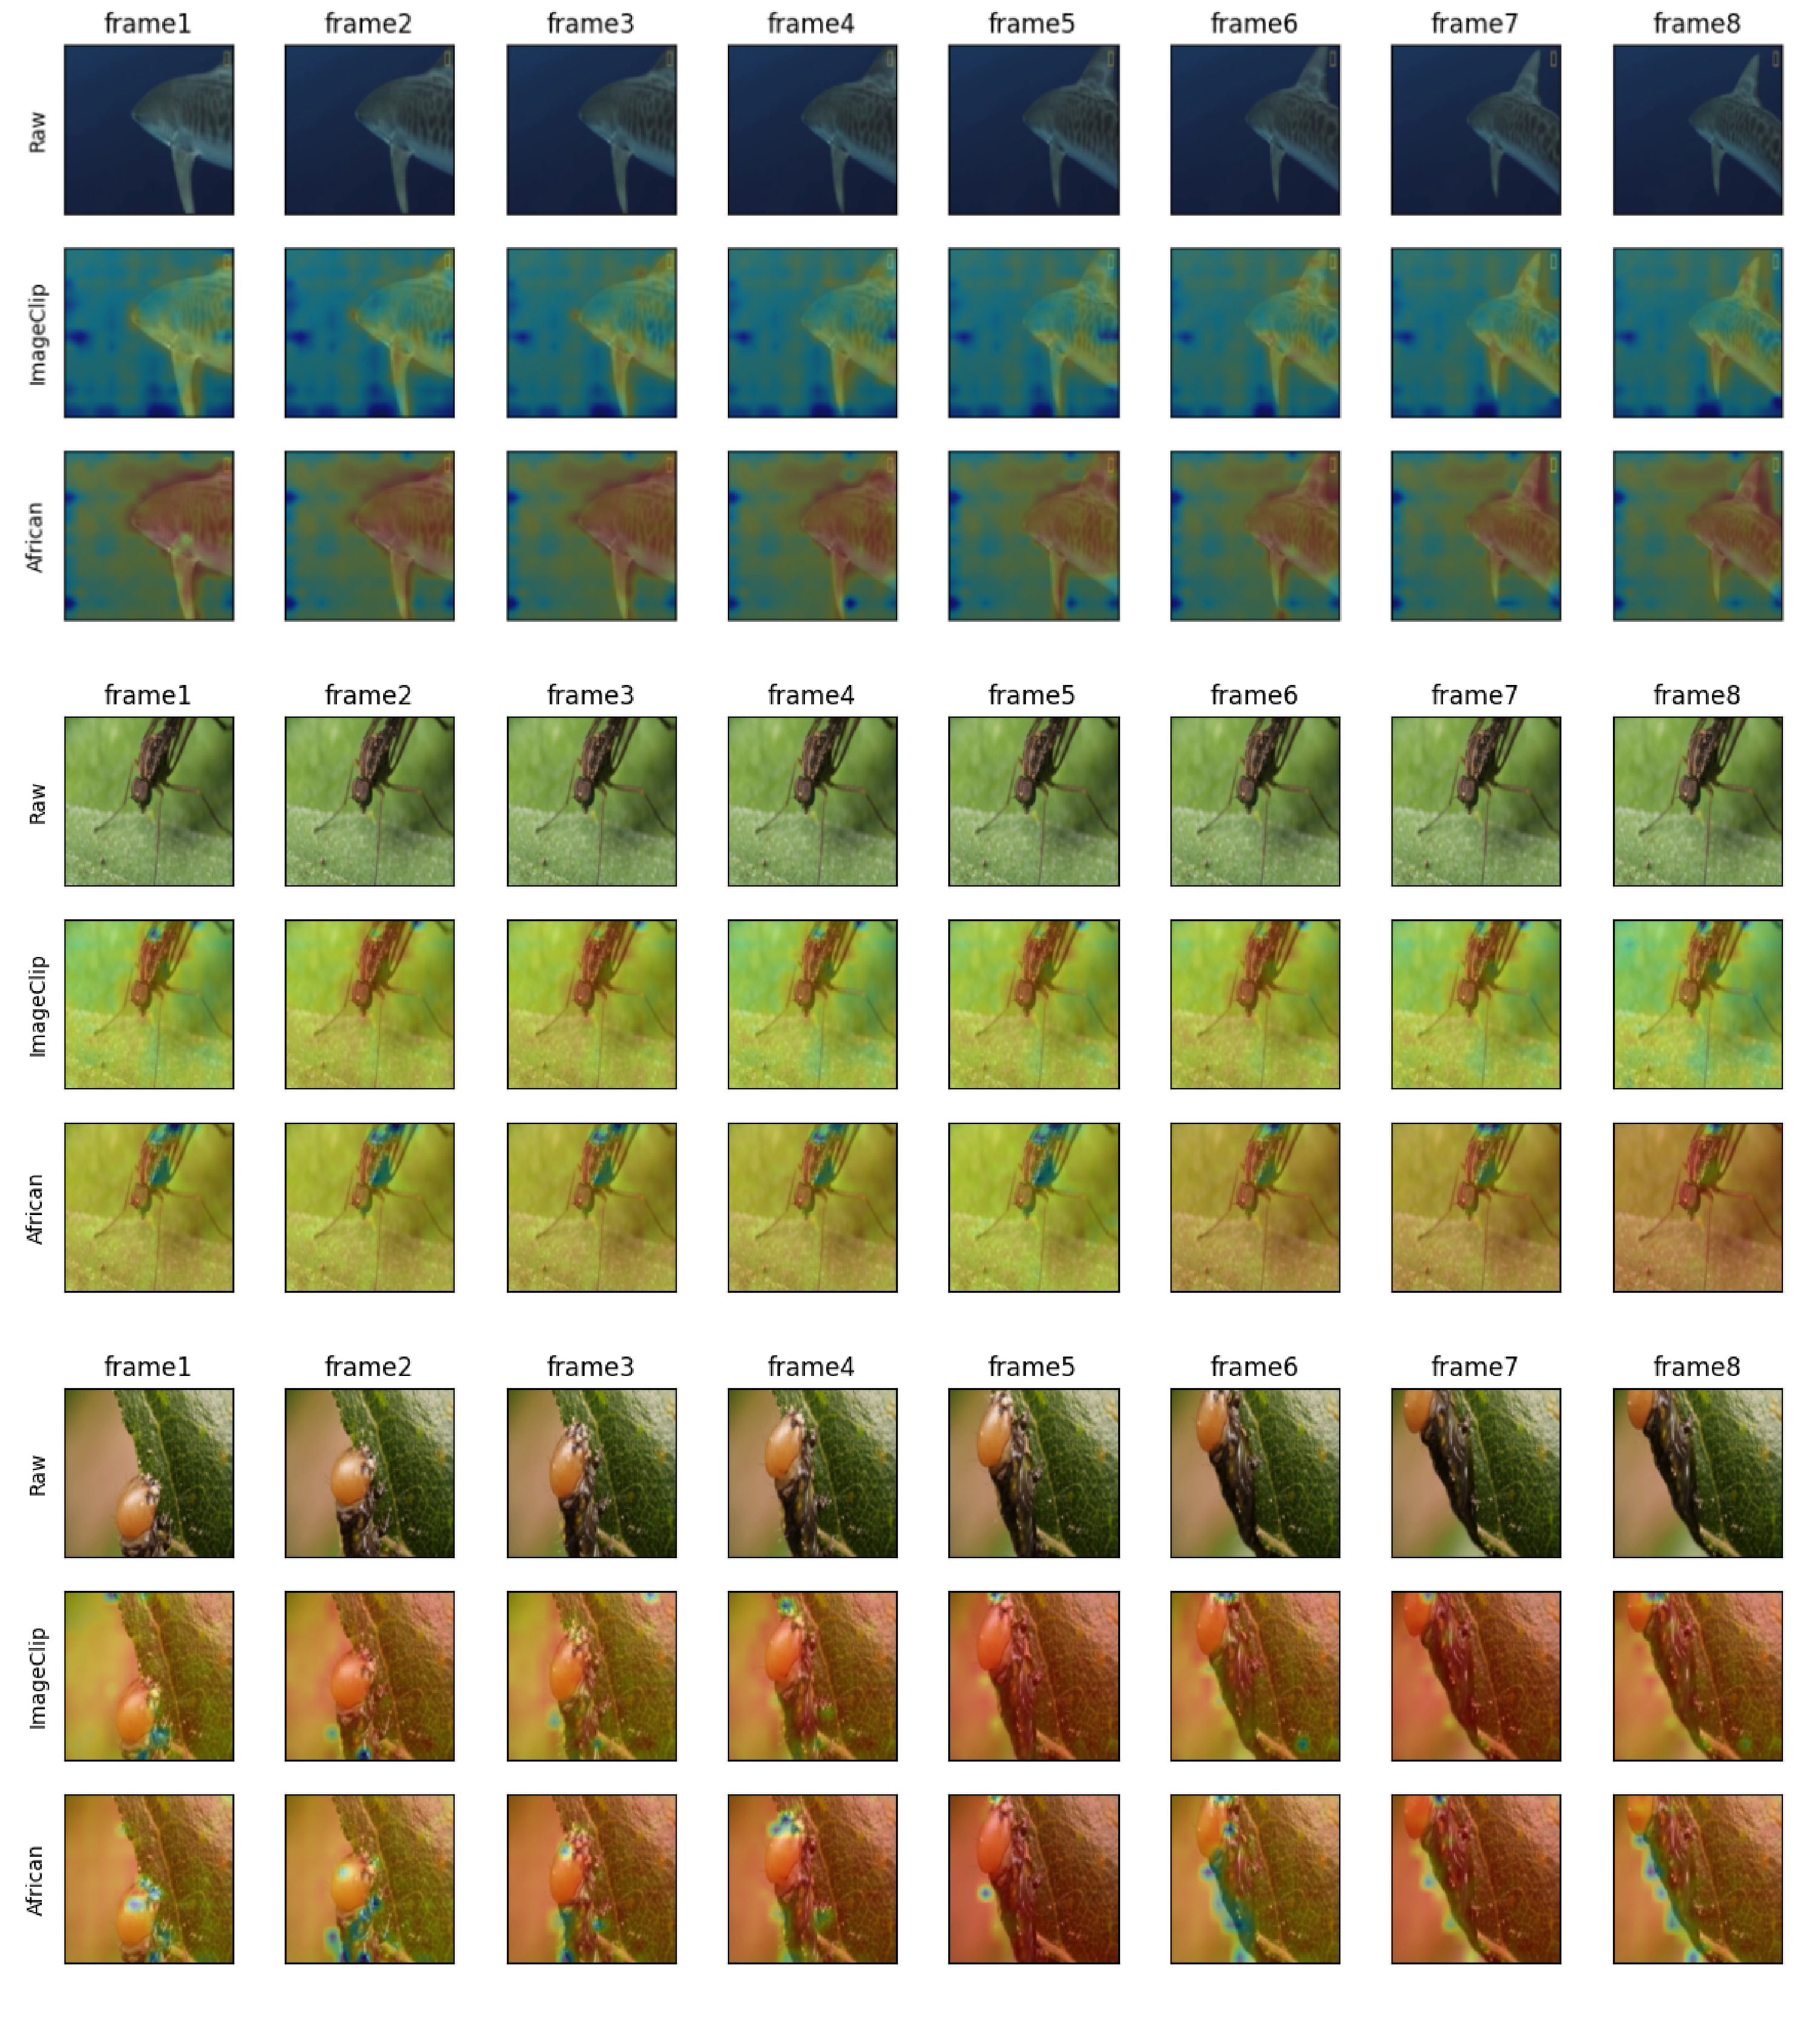
\includegraphics[width=1.0\textwidth]{assets/imgs/5_4_AttentionMaps_1}
    \caption[Attention Map 1]{The attention map for three videos. The first row is the input video, the second row is the attention map of the w/o-AFRICAN model, and the third row is the attention map of the with-AFRICAN model.}
    \label{fig:attnmap1}
\end{figure}

\begin{figure}[ht]
    \centering
    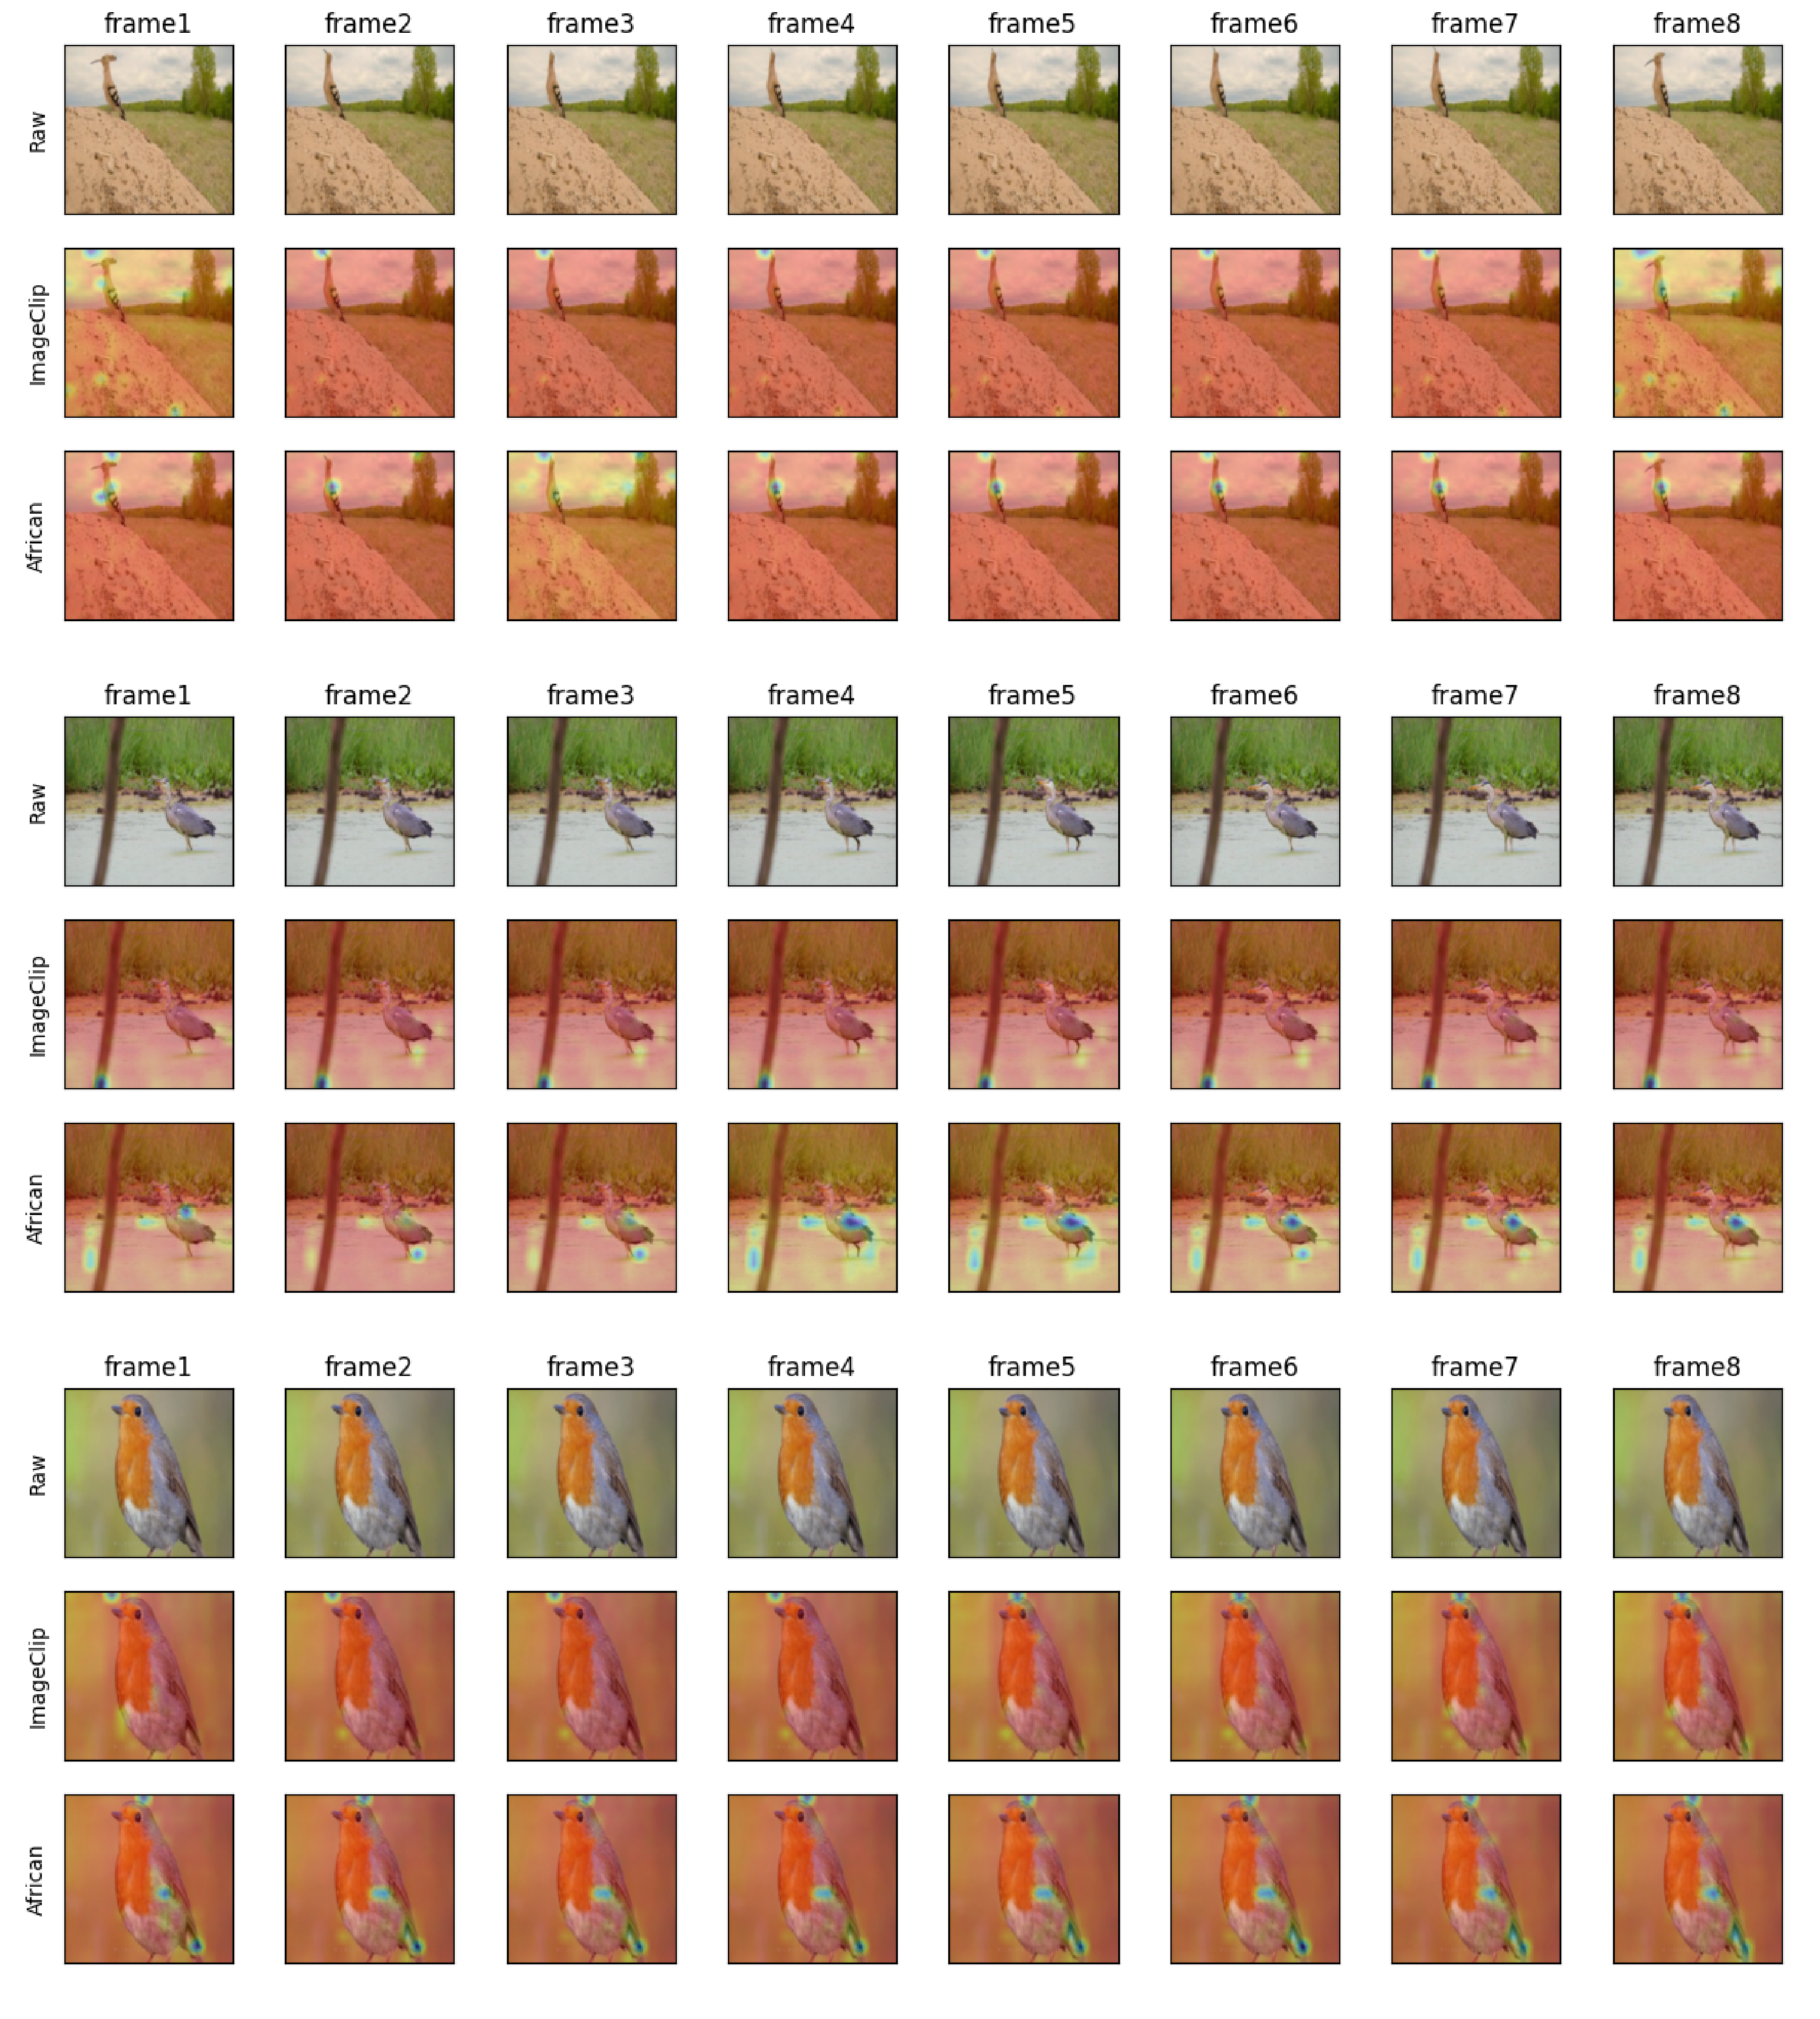
\includegraphics[width=1.0\textwidth]{assets/imgs/5_4_AttentionMaps_2}
    \caption[Attention Map 1]{The same with Figure \ref{fig:attnmap1} for another three videos.}
    \label{fig:attnmap2}
\end{figure}







\subsection{AFRICAN for Action Recognition}
The AFRICAN model for action recognition denoted as AFRICAN-AR, the structure is illustrated in Figure \ref{fig:modelstructaf_ar}, which is trained with a binary cross-entropy loss and adamw optimizer, using a learning rate of 0.00015 on a single A100 GPU. Since the video clip module of the InterVideo takes longer to converge, as illustrated in Figure \ref{fig:tp_backbone} where the IC model does not improve after Epoch 40, I train the model for 40 epochs for the experiment. The mAP is also used as the evaluation metric in this task.

The results for action recognition at Epoch 40 are presented in Table \ref{tab:allresults40}, and the results at the best epoch are shown in Table \ref{tab:allresultsbest}. With the stream of AFRICAN pretrained weights, the AFRICAN-AR are able to outperform the other models in all measured aspects at Epoch 40, with an overall mean Average Precision (mAP) of 54.02\%. At the best epoch, the AFRICAN-AR model generally performs best with an overall mAP of 55.08\%, except in the Tail metric, where IC takes the lead with 48.96\%.


\begin{table}[h]
    \centering
    \caption{Results of action recognition (Epoch 40)}
    \label{tab:allresults40}
    \begin{tabular}{lllll}
        \toprule
        \multirow{2}{*}{Models} & \multicolumn{4}{c}{mAP} \\
        \cmidrule{2-5} 
        {} & Overall & Head  & Middle & Tail \\
        \midrule
        CARe          & 30.55   & 63.33 & 38.62 & 25.09 \\
        IC            & 52.33   & 69.53 & 60.52 & 45.79 \\        
        AFRICAN-AR    & \textbf{54.02} & \textbf{73.54} & \textbf{64.38} & \textbf{46.21} \\
        \bottomrule
    \end{tabular}
\end{table}

\begin{table}[h]
    \centering
    \caption{Results of action recognition (Best Epoch)}
    \label{tab:allresultsbest}
    \begin{tabular}{lllll}
        \toprule
        \multirow{2}{*}{Models} & \multicolumn{4}{c}{mAP} \\
        \cmidrule{2-5} 
        {} & Overall & Head  & Middle & Tail \\
        \midrule
        CARe        & 30.55   & 63.33 & 38.62  & 25.09 \\
        IC          & 54.67   & 71.72 & 63.31 & \textbf{48.96} \\
        AFRICAN     & \textbf{55.08} & \textbf{74.16} & \textbf{65.60} & 47.75 \\
        \bottomrule
    \end{tabular}
\end{table}






% % Need ICs1_B
% % Need ICAFs1_B
% % Need ICs1loh B (failed)
% % Need ICs1loh F
% % Need VCs1dd_bs008 F
% % Need VCs1dd_bs032 F
% % Need VCs1_B no text embedding proj


% TODO
% 0. evaluate on the best score
% 1. Add VC vs. IC Section of Ablation Study (Further training 2 epochs for VCdd)
% 2. Update Table for Backbone Selection (wait ICs1_B)
% 3. Update Table For AFRICAN-AR (wait ICAFs1_B)
% 4. (Time Permmited) Add FocalLoss of IC Section Ablation Study
% 4. (Time Permmited) Add batch size section of Ablation Study (VCs1dd_bs008_B and VCs1dd_bs008_B)

